
\errorcontextlines=200

\documentclass[finalspec]{sbmlpkgspec}
%% \documentclass[draftspec]{sbmlpkgspec}
\usepackage{microtype}
\usepackage{color}
\usepackage{todonotes}
\usepackage[color]{changebar}
\usepackage{xcolor}
\usepackage{soul}
\usepackage{subcaption}
\usepackage{longtable}

% Make changebars switchable to allow faster compilation:
%\def\fullchangebars{} % comment this out to simplify changebars and speed up compilation

% Macros just for this document:

\newcommand{\sbmlpkg}{\texorpdfstring{%
    \textls[-25]{\textsc{SBMLPkgSpec}}}{%
    \textsc{SBMLPkgSpec}}\xspace}
\newcommand{\sbmlpkghead}{\texorpdfstring{%
    \textls[-50]{\textsc{SBMLPkgSpec}}}{%
    \textsc{SBMLPkgSpec}}\xspace}
\newcommand{\sbmlpkgfile}{\literalFont{sbmlpkgspec.cls}\xspace}
\newcommand{\latex}{\LaTeX{}\xspace}
\newcommand{\tex}{\TeX{}\xspace}
\newcommand{\distURL}{http://sourceforge.net/projects/sbml/files/specifications/tex}
\newcommand{\srcURL}{https://sbml.svn.sourceforge.net/svnroot/sbml/trunk/project/tex/sbmlpkgspec}
\newcommand{\webURL}{http://sbml.org/Documents/Specifications/The_SBMLPkgSpec_LaTeX_class}
\newcommand{\cmd}[1]{\literalFont{\textbackslash #1}}

% Custom latex listing style, for use with the listings package.  The default
% highlights far too many things, IMHO.  This keeps it simple and only adjusts
% the appearance of comments within listings.

\lstdefinelanguage{mylatex}{%
  morekeywords={},%
  sensitive,%
  alsoother={0123456789$_},%$
  morecomment=[l]\%%
}[keywords,tex,comments]

\lstdefinestyle{latex}{language=mylatex}


%Command to format the listings containing SBOL RDF/XML serialization examples
\newcommand{\lstsetsbol}{
 \lstset{language=labop,
        tabsize=2
 }
}

%Commands to format SBOL terms in the document

% Use sbolheading when you are referencing a data model class/field in a
% section heading.
\newcommand{\labopheading}[1]{\texttt{#1}}

% Use sbol when you are referencing a LabOP data model class/field in text.
\newcommand{\labop}[1]{\texttt{\hyperref[sec:labop:#1]{#1}}}

% Use sbolmult for SBOL fields that appear in multiple classes, for example
% \sbolmult{types:CD}{types}. This ensures the reference links to the correct
% section.
\newcommand{\labopmult}[2]{\texttt{\hyperref[sec:labop:#1]{#2}}}

% Use sbolheading when you are referencing an SBOL data model class/field in a
% section heading.
\newcommand{\umlheading}[1]{\texttt{uml:#1}}

% Use sbol when you are referencing an SBOL data model class/field in text.
\newcommand{\uml}[1]{\texttt{\hyperref[sec:uml:#1]{uml:#1}}}

% Use sbolmult for SBOL fields that appear in multiple classes, for example
% \sbolmult{types:CD}{types}. This ensures the reference links to the correct
% section.
\newcommand{\umlmult}[2]{\texttt{\hyperref[sec:uml:#1]{uml:#2}}}

% Use sbol when you are using a class borrowed from SBOL, this will prepend the "sbol:" prefix as well
\newcommand{\sbol}[1]{\texttt{\hyperref[sec:sbol:#1]{sbol:#1}}}

% Use sbolmult for SBOL fields that appear in multiple classes, for example
% \sbolmult{types:CD}{types}. This ensures the reference links to the correct
% section.
\newcommand{\sbolmult}[2]{\texttt{\hyperref[sec:sbol:#1]{sbol:#2}}}

% Use prov when you are using a class borrowed from Prov-O, this will prepend the "prov:" prefix as well
\newcommand{\prov}[1]{\texttt{\hyperref[sec:prov:#1]{prov:#1}}}

% Use provmult for Prov-O fields that appear in multiple classes, for example
% \sbolmult{hadRole:U}{hadRole}. This ensures the reference links to the correct
% section.
\newcommand{\provmult}[2]{\texttt{\hyperref[sec:prov:#1]{prov:#2}}}

% Use om when you are using a class borrowed from Ontology of Units & Measures, this will prepend the "om:" prefix as well
\newcommand{\om}[1]{\texttt{\hyperref[sec:om:#1]{om:#1}}}

% Use provmult for OM fields that appear in multiple classes, for example
% \sbolmult{hadUnit:M}{hadUnit}. This ensures the reference links to the correct
% section.
\newcommand{\ommult}[2]{\texttt{\hyperref[sec:om:#1]{om:#2}}}

%Command to format external terms in the document
\newcommand{\external}[1]{\texttt{#1}}

% Rarely used. Use refObj you want to put the field in angle brackets.
\newcommand{\refObj}[1]{$\langle$#1$\rangle$}

\setcounter{tocdepth}{5}
\setcounter{secnumdepth}{5}

% -----------------------------------------------------------------------------
% Start of document
% -----------------------------------------------------------------------------

\begin{document}
\packageTitle{\latex LabOP Specifications}
\packageVersion{Version 1.0-alpha}
\packageVersionDate{TBD, 2021}

\title{Laboratory Open Protocol language \texorpdfstring{\\[3pt]}{}\mbox{(LabOP) Version~1.0.0-alpha}}

\author{
\begin{tabular}{l>{\hspace*{15pt}}r}
Bryan Bartley & \emph{Raytheon BBN Technologies, USA} \\
Jacob Beal & \emph{Raytheon BBN Technologies, USA}\\   
Daniel Bryce & \emph{SIFT, USA}\\
Robert P. Goldman & \emph{SIFT, USA}\\
Benjamin Keller & \emph{University of Washington, USA}\\
Peter Lee & \emph{Strateos, USA}\\
Joshua Nowak & \emph{Strateos, USA}\\
Miles Rogers & \emph{Raytheon BBN Technologies, USA}\\   
Mark Weston & \emph{Netrias, USA}\\
Additional authors & from contributing organizations\\
\end{tabular}\\
}

\maketitlepage

\maketableofcontents

% -----------------------------------------------------------------------------
\section{Purpose}
% -----------------------------------------------------------------------------

Laboratory protocols are critical to biological research and development, but can be difficult to communicate or reproduce due to the differences in context, skills, and resources between different projects, investigators, and organizations.
The Protocol Activity Markup Language (PAML) aims to address this problem by providing a data model for description of laboratory protocols that is unambiguous enough for precise interpretation and automation, yet simultaneously abstract enough to support reuse and adaptation.

It behoves us to unpack the notion of replicability further, in order to better undestand the requirements on PAML as an artifact.  What does it mean to be ``unambiguous enough for precise interpretation and automation'' and `` support reuse and adaptation''? More specifically, what \emph{computational tasks} must PAML support?  We list here a bare minimum set of tasks; there are opportunities to add many more:

\begin{description}
\item[Instantiation] An \emph{abstract} protocol specifies a \emph{recipe} for scientific investigation.  A concrete \emph{instance of} a protocol is an execution of the recipe at a specific time and place, on a specific set of equipment, etc.  This implies at least two representational requirements:
  \begin{description}
  \item[Instantiation Proper] We must be able to create some persistent data structure that represents the protocol instance.
  \item[Derivation] We must be able to represent the relationship between the protocol instance and the recipe from which it is derived.
  \end{description}

\item[Modification] We must be able to record modifications made to the original recipe, for example, to enable it to be executed at a lab with different equipment from the lab at which it was originated, to enable the protocol to be scaled up or scaled down, etc.

A use pattern that may end up being common is to have a protocol be ``too strict" (too specific) to be instantiated in a lab, and thus need modification. Rather than the modification being a patch, as one might do in programming, however, the user would generalize the original protocol \emph{into a new protocol} that is a generalization allowing it to be instantiated in both the labs where it was originated \emph{and} in new labs.  This new protocol would be released as an updated version of the existing protocol.

In this context, the term ``modification'' is intended to refer to \emph{tracking modifications}: what is required is a combination of \emph{versioning} and \emph{provenance tracking}.  A method for computing understandable version differences would also be part of this high level task, which encompasses ongoing development and versioning of the protocol.

A key requirement here will be maintaining information about the \emph{actual version} of the protocol used in an experiment, and underlying a particular dataset, in order that versioning issues not cause incorrect data interpretation.

\item[Metadata markup] A PAML protocol description (possibly with some ancillary information supplied by, e.g., an OPIL document, the container ontology, etc.) should support automatically tagging with metadata data that are collected in the course of protocol execution, \emph{to the extent lab automation at the executing lab supports this}.  For example, a protocol that collects flow cytometry data on samples of different strains under varying growth conditions, should support automatically recording the strain, growth conditions, time of data collection, calibration, etc. of these measurements.
\item[Planning and scheduling] Lab resources are valuable and scarce, and some organizations will want to be able to optimize their use. To do so, PAML should support (at least) extraction of resource requirements from activities in the protocol, and estimated durations.  Note that \emph{what} resource requirements and duration estimates are required will likely be a function of both the protocol and the lab.  What resources are limited, and must be considered in a planner or scheduler, versus those that can be effectively treated as unlimited, will vary by lab.  Management styles will also vary between organizations.
\item[Verification] Authoring a formal protocol in PAML requires substantial mental effort, and the usefulness of the corresponding artifacts can be compromised if they are ill-formed or erroneous.  Supporting protocol authors in achieving correctness is an important goal. Some of this will fall onto the shoulders of those building PAML support tools, however the specification itself must provide guidance as to what it means for a protocol to be complete, consistent, etc.
\item[Mapping protocols to labs] PAML aims to support replication in part by providing automated support for mapping protocols developed at one lab onto another.  We suspect that for some time to come this will be at best a semi-automated process, and like verification, this task will fall heavily on those who provide tool support for PAML users.  However, also as for verification, the PAML specification must say what it means to perform this task correctly -- what a protocol specification truly requires, what aspects can safely be varied, and which must be honored.  This task is closely tied to the task of verification.
\item[Authoring derived works] As with most complex formal artifacts (programs, spreadsheets, etc.), we confidently expect that few users will create new protocols from an entirely blank slate.  Instead, most will take an existing protocol, copy it, and edit the copy.  PAML must support this mode of operation.  Key issues here are which component structures can be incorporated by reference, and which must be copied instead.  Tracking the relationship between an original protocol, and protocols that have branched from it would also be desirable, in order to support, for example, propagating fixes from a root protocol to others.

\item[Protocol maintenance] Closely related to the tasks of ``Modification,'' and ``Derived works'' are the ongoing development, repair, and versioning of a protocol.

\end{description}

Where possible, PAML builds on other existing standards.
In particular, PAML uses the Unified Modeling Language (UML) version 2.5.1~\citep{uml251} to describe the organization of actions in a protocol, the Synthetic Biology Open Language (SBOL) version 3~\citep{SBOL3} to describe biological materials in terms of combinations of strains, media, etc., and uses the Ontology of Units of Measure (OM)~\citep{om2} to describe parameters with physical units.
As a foundation, PAML uses existing Semantic Web practices and resources, such as \emph{Uniform Resource Identifiers} (\paml{URI}s) and ontologies, to unambiguously identify and define biological system elements.
and to provide serialization formats for encoding this information in electronic data files, as well as the SBOL approach to closure in reasoning about knowledge.
This approach also allows PAML to be extended with additional custom information for particular uses and deployments.

Note, however, that PAML intentionally does not provide explicit guarantees about transfer or replicability of protocol executions. 
Likewise, PAML is agnostic to any details of computer networking used to discover or share protocols.
PAML focuses only on representing the minimal information required for an unambiguous specification of what is believed to be important in the execution of a protocol.


%%% Local Variables:
%%% mode: latex
%%% TeX-master: "paml"
%%% End:


%\input{overview}

% -----------------------------------------------------------------------------
\section{Conventions}
% -----------------------------------------------------------------------------

This section provides some preliminary information to aid in the understanding of the specification.
The PAML data model is specified using Unified Modeling Language (UML) 2.5 diagrams~\citep{uml251}. This section reviews terminology conventions, the basics of UML diagrams, and our naming conventions.

\subsection{Terminology Conventions}

This document indicates requirement levels using the controlled vocabulary specified in \href{https://tools.ietf.org/html/rfc2119}{IETF RFC 2119}.
In particular, the key words ``MUST'', ``MUST NOT'', ``REQUIRED'', ``SHALL'', ``SHALL NOT'', ``SHOULD'', ``SHOULD NOT'', ``RECOMMENDED'', ``MAY'', and ``OPTIONAL'' in this document are to be interpreted as described in RFC 2119.

\begin{itemize}
\item The words ``MUST'', ``REQUIRED'', or ``SHALL'' mean that the item is an absolute requirement.
\item The phrases ``MUST NOT'' or ``SHALL NOT'' mean that the item is an absolute prohibition.
\item The word ``SHOULD'' or the adjective ``RECOMMENDED'' mean that there might exist valid reasons in particular circumstances to ignore a particular item, but the full implications need to be understood and carefully weighed before choosing a different course.
\item The phrases ``SHOULD NOT'' or ``NOT RECOMMENDED'' mean that there might exist valid reasons in particular circumstances when the particular behavior is acceptable or even useful, but the full implications needs to be understood and the case carefully weighed before implementing any behavior described with this label.
\item The word ``MAY'' or the adjective ``OPTIONAL'' mean that an item is truly optional.
\end{itemize}

\subsection{UML Diagram Conventions}
\label{sec:umldiagrams}

The types of data modeled by PAML are commonly referred to as {\em classes}, especially when discussing the details of software implementation. Each PAML class can be instantiated by many PAML objects. These objects MAY contain data that differ in content, but they MUST agree on the type and form of their data as dictated by their common class. Classes are represented in UML diagrams as rectangles labeled at the top with class names (see \ref{fig:uml_sampler} for examples).

\begin{figure}[ht]
\begin{center}
  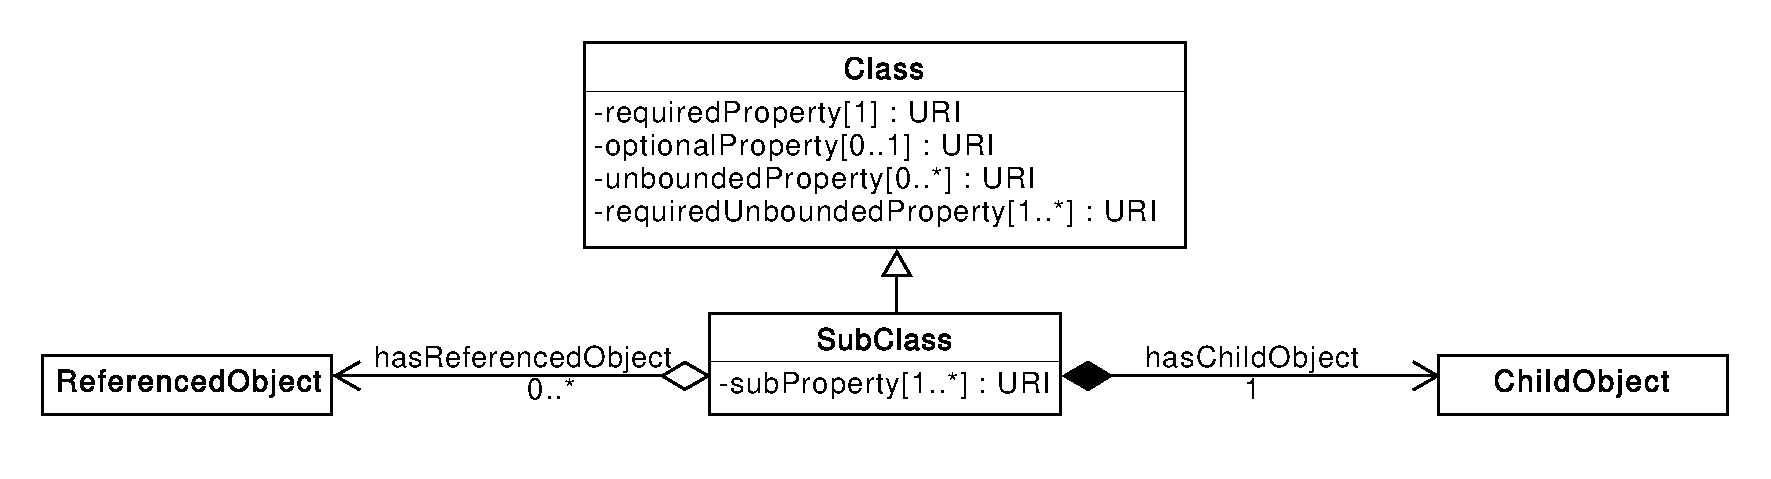
\includegraphics[width=\textwidth]{figures/uml_sampler.pdf}
\caption{Examples of UML diagram conventions used in this document}
\label{fig:uml_sampler}
\end{center}
\end{figure}

Classes can be connected to other classes by association properties, which are represented in UML diagrams as arrows. These arrows are labeled with data cardinalities in order to indicate how many values a given association property can possess (see below). The remaining (non-association) properties of a class are listed below its name. Each of the latter properties is labeled with its data type and cardinality.

In the case of an association property, the class from which the arrow originates is the owner of the association property. A diamond at the origin of the arrow indicates the type of association.
Open-faced diamonds indicate shared aggregation, also known as a reference, in which the owner of the association property exists independently of its value.

By contrast, filled diamonds indicate composite aggregation, also known as a part-whole relationship, in which the value of the association property MUST NOT exist independently of its owner.
In addition, in the PAML data model, it is REQUIRED that the value of each composite aggregation property is a unique PAML object (that is, not the value for more than one such property).
Note that in all cases, composite aggregation is used in such a way that there SHOULD NOT be duplication of such objects.
Such objects are also commonly referred to as ``child'' objects, and their owning objects as ``parent'' objects.

All PAML properties are labeled with one of several restrictions on data cardinality. These are:

\begin{itemize}

\item $1$ - REQUIRED: there MUST be exactly one value for this property.

\item $0 \ldots 1$ - OPTIONAL: there MAY be a single value for this property, or it MAY be absent.

\item $0 \ldots *$ - zero or more: there MAY be any number of values for this property, including none.

\item $1 \ldots *$ - REQUIRED, one or more: there MAY be any number of values for this property, as long as there is at least one.

\item $n \ldots *$ - at least: there MUST be at least $n$ values for this property.

\end{itemize}

Finally, classes can inherit the properties of other classes. Inheritance relationships are represented in UML diagrams as open-faced, triangular arrows that point from the inheriting class to the inherited class. Some classes in the PAML data model cannot be instantiated as objects and exist only to group common properties for inheritance. These classes have italicized names and are known as abstract classes.

\subsection{Naming and Typographic Conventions}
\label{sec:nameconventions}

PAML classes are named using upper ``camel case,'' meaning that each word is capitalized and all words are run together without spaces, e.g., \paml{Protocol}.
Properties, on the other hand, are named using lower camel case, meaning that they begin lowercase but if they consist of multiple words, all words after the first begin with an uppercase letter (e.g., \paml{hasActivity}).

PAML properties are always given singular names irrespective of their cardinality, e.g., \paml{hasActivity} is used rather than \external{hasParameters} even though a \paml{Protocol} can have multiple parameters.
This is because each relation can potentially stand on its own, irrespective of the existence of others in the set.

Two conventions are used for property names, {\tt name} and {\tt hasName}.  
When a property is pointing to a class using the same name, it uses the {\tt hasName} convention (e.g., the \paml{Protocol} class uses \paml{hasActivity} to point to a \paml{Activity} object).
When the property uses a different name than the class of the object it points to, it uses the {\tt name} convention instead (e.g., the \paml{Protocol} class uses \paml{inputActivity} to point to an input \om{Activity} object).


% -----------------------------------------------------------------------------
\section{SBOL Imports: Identifiers, Primitive Types, and Classes}
% -----------------------------------------------------------------------------

PAML builds on the Synthetic Biology Open Language (SBOL) version 3~\citep{SBOL3} in several ways:
\begin{itemize}
\item PAML uses the same conventions as SBOL for URIs and types.
\item PAML uses the SBOL base classes \sbol{Identified} and \sbol{TopLevel} as parents for all PAML classes.
\item PAML uses SBOL classes to describe biological samples in terms of combinations of strains, media, etc.
\item PAML makes use of the same external measurement ontology as SBOL, the Ontology of Units of Measure (OM)~\citep{om2}.
\end{itemize}

In order to make this document more self-contained, this section repeats the material from the SBOL specification on conventions and SBOL base classes.
A summary is also provided for key SBOL and OM classes; for complete documentation, see the SBOL specification.
In case of conflict between any material in this section and the SBOL specification, the SBOL specification should be held correct.

\subsection{Uniform Resource Identifiers}
\label{sec:URIstructure}

As PAML is built upon the Resource Description Framework (RDF), all class instances are identified by a Uniform Resource Identifier (URI).  In the PAML data model, the value of an association property MUST be a \paml{URI} or set of \paml{URI}s that refer to PAML objects belonging to the class at the tip of the arrow.  Every \sbol{Identified} object's URI MUST be globally unique among all other \sbol{Identified} object URIs. It is also highly RECOMMENDED that the \paml{URI} structure follows the recommended best practices for compliant \paml{URI}s specified in \ref{sec:compliant}.

Whenever a \sbol{TopLevel} object's URI is a URL (e.g., following the conventions of HTTP(S) rather than a UUID), its structure MUST comply with the following rules:

\begin{itemize}

 \item A \sbol{TopLevel} URL MUST use the following pattern:
  \texttt{[namespace]/[local]/[displayId]},  where \texttt{namespace} and \sbol{displayId} are required fragments, and the \texttt{local} fragment is an optional relative path.
  
  	For example, a \paml{Protocol} might have the URL~\path{https://igem.org/protocols/OD/calibration_2018}, where \texttt{namespace} is \path{https://igem.org}, \texttt{local} is \path{protocols/OD}, and \sbol{displayId} is \path{calibration_2018}.

  \item A \sbol{TopLevel} object's URL MUST NOT be included as prefix for any other \sbol{TopLevel} object.
  
  	For example, the \path{run102} \paml{ProtocolExecution} object cannot have a URL of \path{https://igem.org/protocols/OD/calibration_2018/run102}, since the \path{https://igem.org/protocols/OD/calibration_2018} prefix is already used as a URL for a \paml{Protocol} object.

  \item The URL of any child or nested object MUST use the following pattern:\texttt{[parent]/[displayId]}, where \texttt{parent} is the URL of its parent object.
	Multiple layers of child objects are allowed using the same\\ \texttt{[parent]/[displayId]} pattern recursively.
	
	For example, a \uml{CallBehaviorAction} object owned by the \path{calibration_2018} \paml{Protocol} and having a \sbol{displayId} of \texttt{CallBehaviorAction1} will have a URL of \path{https://igem.org/protocols/OD/calibration_2018/CallBehaviorAction1}.
	Similarly, if the \texttt{CallBehaviorAction1} object has a \uml{InputPin} child object with a \sbol{displayId} of \texttt{InputPin1}, then that object will have the URL\\ \path{https://igem.org/protocols/OD/calibration_2018/CallBehaviorAction1/InputPin1}.
  \end{itemize}

\subsubsection{Compliant URIs}
\label{sec:compliant}

Maintaining unique URIs for objects can be challenging.  Compliant URIs follow a set of rules that simplify this challenge.

Compliant URIs for \sbol{TopLevel} objects MUST conform to the following pattern:
\begin{quotation} 
\refObj{namespace}/\refObj{collection\_structure}/\refObj{displayId}
\end{quotation}

The \refObj{namespace} token MAY further decompose into \refObj{domain}/\refObj{root} tokens. The \refObj{root} and \refObj{collection\_structure} tokens may optionally be omitted; alternatively, they may consist of an arbitrary number of delimiter-separated layers. Note that this pattern means that SBOL-compliant \paml{URI}s can be automatically decomposed with the aid of a \sbol{TopLevel} object's \sbol{hasNamespace} property. SBOL-compliant objects can be easily remapped into new namespaces by changing only the \refObj{namespace}.

Consider, for example, the SBOL-compliant \paml{URI}:
\begin{quote}``https://igem.org/engineering/protocols/platereader/OD/calibration\_2018''\end{quote} 
for a \sbol{Component} with a \sbol{hasNamespace} value ``https://igem.org/engineering/protocols''.
This \paml{URI} can be decomposed as follows:
\begin{quote} 
namespace: ``https://igem.org/engineering/protocols'' \linebreak
domain: ``https://igem.org'' \linebreak
root: ``engineering/protocols'' \linebreak
collection: ``platereader/OD'' \linebreak
displayId: ``calibration\_2018'' \linebreak
\end{quote}

SBOL-compliant URIs also facilitate auto-construction of child objects with unique \paml{URI}s. 
Child objects of \sbol{TopLevel} objects with compliant \paml{URI}s MUST conform to the following pattern:\\ ``\refObj{parent\_uri}/\refObj{child\_type}\refObj{child\_type\_counter}'' where the \refObj{parent\_uri} refers to the URI of the parent object, the \refObj{child\_type} refers to the SBOL class of the child object, and \refObj{child\_type\_counter} is a unique index for the child object. 
The \refObj{child\_type\_counter} of a new object SHOULD be calculated at time of object creation as 1 + the maximum \refObj{child\_type\_counter} for each \refObj{child\_type} object in the parent (e.g., ``\refObj{parent\_uri}/Parameter7''). 
Note that numbering is independent for each type, so a \paml{Protocol} can have children ``CallBehaviorAction7'' and ``ControlFlow7''.

\subsection{PAML URIs}
 \label{sec:pamlURIs}
  
\todo[inline]{The actual ontology implementations aren't currently versioned correctly, per \url{https://github.com/SD2E/paml/issues/59}}

The PAML namespace, which is \url{http://bioprotocols.org/paml/v1\#}, is used to indicate which entities and properties in an PAML document are defined by PAML. 
For example, the URI of the type \paml{Protocol} is \url{http://bioprotocols.org/paml/v1\#Protocol}. 
This convention is assumed throughout the specification.
The PAML namespace MUST NOT be used for any entities or properties not defined in this specification.

Likewise, because no suitable ontology previously existed for UML 2.5.1~\citep{uml251}, the subset used by PAML is defined within a sibling namespace, \url{http://bioprotocols.org/uml/v251\#}

Other namespaces are also used by PAML, however, notably the SBOL 3 namespace \url{http://sbols.org/v3\#}, as well as other namespaces used by SBOL including Dublin Core~\citep{dcmi2012}), the PROV-O ontology (\url{https://www.w3.org/ns/prov#}), Ontology of Units of Measure (OM), and various biological ontologies.


\subsection{Primitive Data Types}
\label{sec:datatypes}
\label{sec:string}
\label{sec:integer}
\label{sec:long}
\label{sec:float}
\label{sec:boolean}
\label{sec:URI}
\label{sec:literal}

When PAML uses simple ``primitive'' data types such as \paml{string}s or \paml{integer}s, these are defined as the following specific formal types:
\begin{itemize}
\item \paml{string}: \url{http://www.w3.org/2001/XMLSchema\#string}\\
  {\em Example: ``LacI coding sequence''}
\item \paml{integer}: \url{http://www.w3.org/2001/XMLSchema\#integer}\\
  {\em Example: 3}
\item \paml{long}: \url{http://www.w3.org/2001/XMLSchema\#long}\\
  {\em Example: 9223372036854775806}
\item \paml{float}: \url{http://www.w3.org/2001/XMLSchema\#float}\\
  {\em Example: 3.14159}
\item \paml{boolean}: \url{http://www.w3.org/2001/XMLSchema\#boolean}\\
  {\em Example: \external{true}}
\end{itemize}

The term \paml{literal} is used to denote an object that can be any of the five types listed above.

In addition to the simple types listed above, PAML also uses objects with types \emph{Uniform Resource Identifier} (\paml{URI}). It is important to realize that in RDF, a \paml{URI} might or might not be a resolvable URL (web address).  A \paml{URI} is always a globally unique identifier within a structured namespace.  In some cases, that name is also a reference to (or within) a document, and in some cases that document can also be retrieved (e.g., using a web browser).


\subsection{PAML Types}
\label{sec:pamlTypes}

All PAML objects are given the most specific \external{rdfType} in the PAML namespace (\uri{http://bioprotocols.org/paml/v1\#}) that defines the type of the object.  
Likewise, properties in the PAML namespace should only be used by objects with a PAML \external{rdfType}.

\todo[inline]{We should consider whether we want to maintain this, given UML's love for mix-in classes}
PAML does not use multiple inheritance: all PAML classes are disjoint except with respect to their abstract parent classes.
Accordingly, an object MUST NOT be given two \external{rdfType} properties referring to disjoint classes in the PAML namespace.
An object MAY have redundant \external{rdfType} properties for its parent types, but this is NOT RECOMMENDED.

For example, an object cannot have both the \external{rdfType} of \paml{Protocol} and \paml{SampleCollection}.  Also, a \paml{Protocol} would have this \external{rdfType} and not also include \external{rdfType}s for classes that it inherits from, such as \uml{Activity} and \sbol{Identified}.

The same rules apply to the UML namespace, the SBOL namespace, and all unions thereof.


\subsection{Object Closure and Document Composition}

In RDF, there is no requirement that all of the information about an object be stored in one location.  
Instead, there is a ``open world'' assumption that additional triples describing the object may be acquired at any time.
Documents are allowed to be fragmented and composed in an arbitrary manner, down to their underlying atomic triples, with no consideration for object structure.

This limits the ability to reason about properties of objects and validate the correctness of a model.
For example, it would not be possible to validate that an \sbol{Identified} object has no more than one value for its \sbol{displayId} property, because it would not be possible to determine whether some other document somewhere in the world holds a second value for the property.

SBOL addresses this by adding an object closure assumption that allows stronger reasoning about individual objects and their children, and PAML adopts this convention.
For any given PAML document, if the document contains an \external{rdfType} statement regarding an \sbol{Identified} object $X$, then it is assumed that the document also contains all other property statements about object $X$ as well. 
This enables strong validation rules, since any statement of the form ``$X$ {\it predicate} $Y$'' that is not present can be assumed to be false.
For example, if a document has one value for an object's \sbol{displayId}, then it is valid to conclude that there are no other \sbol{displayId} values, and thus its "zero or one" cardinality requirement is satisfied.

We further assume that any document containing an object also contains all of its child objects.
In other words, the fundamental unit of PAML documents is the \sbol{TopLevel} object, and any document containing a \sbol{TopLevel} also contains the complete set of information necessary to describe that \sbol{TopLevel}---but not necessarily any other \sbol{TopLevel} objects that it refers to.
For example, a document containing an \paml{ProtocolExecution} describing the execution of a protocol is guaranteed to contain every \paml{ActivityEdgeFlow} for the execution, but the document might not contain the \paml{Protocol} that was executed.

A PAML document thus cleaves naturally along the boundaries of \sbol{TopLevel} objects, implying the following set of rules of fragmentation and composition of documents:
\begin{itemize}
\item Any subset of \sbol{TopLevel} objects in a valid PAML document is also a valid PAML document.
\item Any disjoint set of \sbol{TopLevel} objects from different PAML documents MAY be composed to form a new PAML document. The result is not guaranteed to be valid, however, since the composition may expose problems due to the relationships between \sbol{TopLevel} objects from different documents.
\item If two \sbol{TopLevel} objects in different PAML documents have the same identity and and both they and their child objects contain equivalent sets of property assertions, then they MAY be treated as identical and freely merged. 
\item  If two \sbol{TopLevel} objects in different PAML documents have the same identity but different property values, then they MUST be considered different (possibly conflicting) versions, and any merger managed through some version control process.
\end{itemize}


\subsection{SBOL Classes}

PAML classes use \sbol{Identified} and \sbol{TopLevel} as their root classes.
PAML also uses \sbol{Component} to describe biological materials such as strains, reagents, genetic constructs, and media.
This subsection summarizes the minimum information required to use these SBOL classes in PAML; for full details, see the Synthetic Biology Open Language (SBOL) version 3 specification~\citep{SBOL3}

\subsubsection{sbol:Identified}
\label{sec:sbol:Identified}

All PAML- and SBOL-defined classes are directly or indirectly derived from the \sbol{Identified}  abstract class.
This inheritance means that all PAML and SBOL objects are uniquely identified using \paml{URI}s that uniquely refer to these objects within an SBOL document or at locations on the World Wide Web.

As shown in \ref{uml:identified}, the \sbol{Identified} class includes the following properties: \sbol{displayId},  \sbol{name}, \sbol{description}, \prov{wasDerivedFrom}, and \prov{wasGeneratedBy}. 

\begin{figure}[ht]
\begin{center}
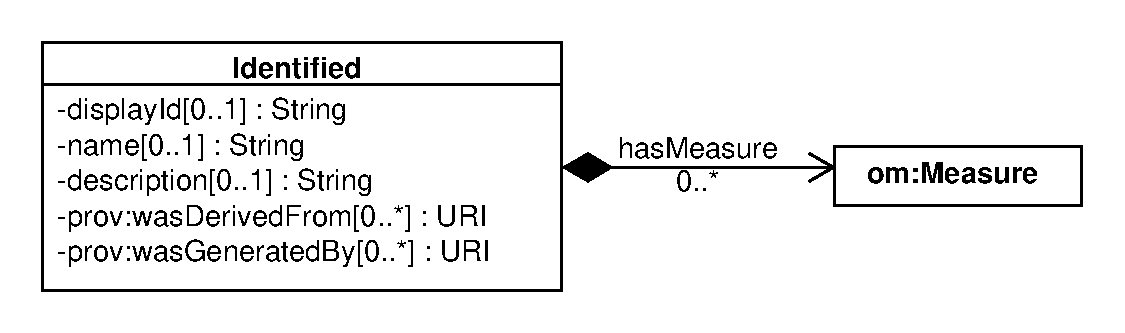
\includegraphics[scale=0.6]{sbol_classes/identified}
\caption[]{Diagram of the \sbol{Identified} abstract class and its associated properties}
\label{uml:identified}
\end{center}
\end{figure}

\begin{itemize}
\item \label{sec:sbol:displayId} 
The \sbol{displayId} property is an OPTIONAL identifier with a data type of \paml{string} (and REQUIRED for objects with URL identifiers). This property is intended to be an intermediate between a URI and the \sbol{name} property that is machine-readable, but more human-readable than the full URI of an object.
If set, its \paml{string} value MUST be composed of only alphanumeric or underscore characters and MUST NOT begin with a digit.

\item \label{sec:sbol:name}
The \sbol{name} property is OPTIONAL and has a data type of \paml{string}. This property is intended to be displayed to a human when visualizing an \sbol{Identified} object.
If an \sbol{Identified} object lacks a name, then software tools SHOULD instead display the object's \sbol{displayId} or URI.

\item \label{sec:sbol:description}
The \sbol{description} property is OPTIONAL and has a data type of \paml{string}. This property is intended to contain a more thorough text description of an \sbol{Identified} object.

\item \label{sec:prov:wasDerivedFrom}
The \prov{wasDerivedFrom} property MAY contain any number of \paml{URI}s. This property is defined by the PROV-O ontology and is located in the \url{https://www.w3.org/ns/prov#} namespace.

\item \label{sec:prov:wasGeneratedBy}
The \prov{wasGeneratedBy} property MAY contain any number of \paml{URI}s. This property is defined by the PROV-O ontology and is located in the \url{https://www.w3.org/ns/prov#} namespace.

\item \label{sec:sbol:hasMeasure}
The \sbol{hasMeasure} property MAY contain any number of \paml{URI}s, each of which refers to a \om{Measure} object that describes a measured parameter for this object.
\end{itemize}

\subsubsection{sbol:TopLevel}
\label{sec:sbol:TopLevel}

\sbol{TopLevel} is an abstract class that is extended by any \sbol{Identified} class that can be found at the top level of a PAML or SBOL document or file.
In other words, \sbol{TopLevel} objects are never nested inside of any other object as a child object.
The \sbol{TopLevel} classes defined in PAML are \paml{Protocol} and \paml{Primitive}. 

\begin{figure}[ht]
\begin{center}
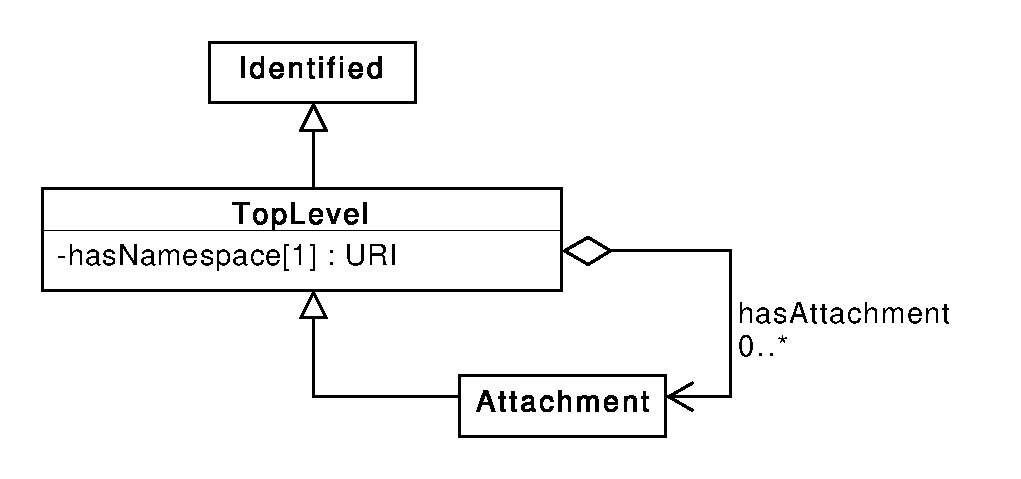
\includegraphics[scale=0.6]{sbol_classes/toplevel}
\caption[]{Classes that inherit from the \sbol{TopLevel} abstract class.}
\label{uml:toplevel}
\end{center}
\end{figure}

\begin{itemize}
\item \label{sec:sbol:hasNamespace}
The \sbol{hasNamespace} property is REQUIRED and MUST contain a single \paml{URI} that defines the namespace portion of URLs for this object and any child objects.
If the URI for the \sbol{TopLevel} object is a URL, then the URI of the \sbol{hasNamespace} property MUST prefix match that URL.

\item 
\label{sec:sbol:hasAttachment}
The \sbol{hasAttachment} property MAY have any number of \paml{URI}s, each referring to an \external{sbol:Attachment} object.
\end{itemize}


\subsubsection{sbol:Component}
\label{sec:sbol:Component}

The \sbol{Component} class represents the structural and/or functional entities of a biological design. 
In PAML, this is primarily used to represent the design of experimental samples as combinations of entities such as strains, genetic constructs, media, inducers, etc.

As shown in \ref{uml:component}, the \sbol{Component} class describes a design entity using a number of different properties.
In many PAML usages, however, a \sbol{Component} will simply be used as a pointer to an external description of a material to be manipulated, and the only property required for interpreting PAML will be \sbolmult{type:C}{type}.

\begin{figure}[ht]
\begin{center}
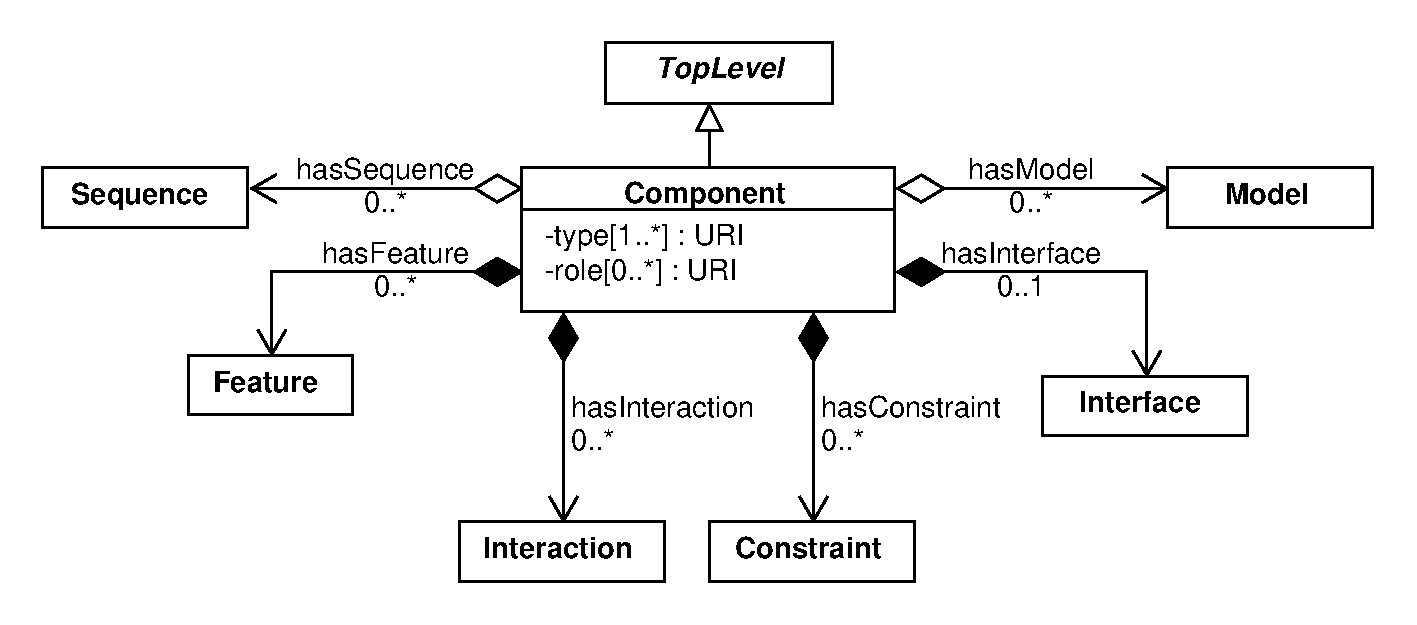
\includegraphics[scale=0.6]{sbol_classes/component}
\caption[]{Diagram of the \sbol{Component} class and its associated properties.}
\label{uml:component}
\end{center}
\end{figure} 

\begin{itemize}
\item \label{sec:sbol:type:C}
The \sbolmult{type:C}{type} property MUST have one or more \paml{URI}s specifying the category of biochemical or physical entity (for example DNA, protein, or simple chemical) that a \sbol{Component} object represents.

\item \label{sec:sbol:hasFeature}
The \sbol{hasFeature} property MAY have any number of \paml{URI}s, each referencing a \sbol{Feature} object. Each \sbol{Feature} represents a specific occurrence of a part, subsystem, or other notable aspect within that design, such as an ingredient in the composition of a growth medium.
\\{\em This is not typically required for specifying protocols in PAML.}

\item \label{sec:sbol:role:C}
The \sbolmult{role:C}{role} property MAY have any number of \paml{URI}s, which MUST identify terms from ontologies that are consistent with the \sbolmult{type:C}{type} property of the \sbol{Component}. 
\\{\em This is not typically required for specifying protocols in PAML.}

\item \label{sec:sbol:hasSequence:C}
The \sbolmult{hasSequence:C}{hasSequence} property MAY have any number of \paml{URI}s, each referencing a \external{sbol:Sequence} object.  These objects define the primary structure or structures of the \sbol{Component}.
\\{\em This is not typically required for specifying protocols in PAML.}

\item \label{sec:sbol:hasConstraint}
The \sbol{hasConstraint} property MAY have any number of \paml{URI}s, each referencing a \external{sbol:Constraint} object.
These objects describe, among other things, any restrictions on the relative, sequence-based positions and/or orientations of the \sbol{Feature} objects contained by the \sbol{Component}, as well as spatial relations such as containment and identity relations.
\\{\em This is not typically required for specifying protocols in PAML.}

\item \label{sec:sbol:hasInteraction}
The \sbol{hasInteraction} property MAY have any number of \paml{URI}s, each referencing an \external{sbol:Interaction} object describing a behavioral relationship between \sbol{Feature}s in the \sbol{Component}.
\\{\em This is not typically required for specifying protocols in PAML.}

\item \label{sec:sbol:hasInterface}
The \sbol{hasInterface} property is OPTIONAL and MAY have a \paml{URI} referencing an \external{sbol:Interface} object that indicates the inputs, outputs, and non-directional points of connection to a \sbol{Component}.
\\{\em This is not typically required for specifying protocols in PAML.}

\item \label{sec:sbol:hasModel}
The \sbol{hasModel} property MAY have any number of \paml{URI}s, each referencing a \external{sbol:Model} object that links the \sbol{Component} to a computational model in any format.
\\{\em This is not typically required for specifying protocols in PAML.}
\end{itemize}

\subsection{PROV-O}

The PROV-O ontology (\url{https://www.w3.org/ns/prov#}) defines a complementary data model that is leveraged by PAML to describe provenance.
PAML builds on PROV-O to represent the execution of \paml{Protocol} workflows and the \paml{Primitive} behaviors that they comprise.
A subset of PROV-O, already adapted for use with SBOL, is used for this purpose by PAML as well.

The key class used is \prov{Activity}, which serves as a parent class for \paml{BehaviorExecution} records, along with \prov{Association} and \prov{Agent}, which are used to record the entity carrying out an execution.
We repeat here only the key portions referenced in this specification.

\subsubsection{prov:Activity}
\label{sec:prov:Activity}

An \prov{Activity} is used to describe how different \prov{Agent}s and other entities were used. An \prov{Activity} is linked through a \prov{qualifiedAssociation} to \prov{Association}s, to describe the role of agents.
Each \prov{Activity} includes optional \prov{startedAtTime} and \prov{endedAtTime} properties. 

\begin{itemize}
\item \label{sec:type:Activity}
An \prov{Activity} MAY have one or more \pamlmult{type:Activity}{type} properties, each of type \paml{URI} that explicitly specifies the type of the provenance \prov{Activity} in more detail.

\item \label{sec:prov:startedAtTime}
The \prov{startedAtTime} property is OPTIONAL and contains a DateTime value, indicating when the activity started.  If this property is present, then the \prov{endedAtTime} property is REQUIRED.

\item \label{sec:prov:endedAtTime}
The \prov{endedAtTime} property is OPTIONAL and contains a DateTime value, indicating when the activity ended.

\item \label{sec:prov:qualifiedAssociation}
An \prov{Activity} MAY have one or more \prov{qualifiedAssociation} properties, each of type \sbol{URI} that refers to an \prov{Association} object.
\end{itemize}

\subsubsection{prov:Association}
\label{sec:prov:Association}

An \prov{Association} is linked to an \prov{Agent} through the \prov{agent} relationship. The \prov{Association} includes the \provmult{hadRole:A}{hadRole} property to qualify the role of the \prov{Agent} in the \prov{Activity}.

\begin{itemize}
\item \label{sec:prov:agent}
The \prov{agent} property is REQUIRED and MUST contain a \paml{URI} that refers to an \prov{Agent} object.

\item \label{sec:prov:hadRole:A}
An \prov{Association} MAY have one or more \provmult{hadRole:A}{hadRole} properties, each of type \paml{URI} that refers to particular term(s) that describes the role of the \prov{Agent} in the parent \prov{Activity}. 
\end{itemize}

\subsubsection{prov:Agent}
\label{sec:prov:Agent}

Examples of agents are a person, organization, or software tool. 
These agents should be annotated with additional information, such as software version, needed to be able to run the same \prov{Activity} again.



\subsection{Ontology of Units of Measure}

In most cases where a number is needed in PAML, that number is a measure with units associated with it.
The Ontology of Units of Measure (OM) (\url{http://www.ontology-of-units-of-measure.org/resource/om-2}) already defines a data model for representing measures and their associated units. 
A subset of OM, already adapted for use with SBOL, is used for this purpose by PAML as well.

The key class used is \om{Measure}, which associates a number with a unit and a biology-related property.
In most cases, it should be possible to use one of the \external{om:Unit} instances already defined by OM; when this is not possible, an appropriate unit can be defined using \external{om:Unit} and \external{om:Prefix} classes.

\subsubsection{om:Measure} \label{sec:om:Measure}

The purpose of the \om{Measure} class is to link a numerical value to a \external{om:Unit}. 

\begin{itemize}
\item \label{sec:om:hasNumericalValue}
The \om{hasNumericalValue} property is REQUIRED and MUST contain a single \paml{float}.

\item \label{sec:om:hasUnit:Measure}
The \ommult{hasUnit:Measure}{hasUnit} property is REQUIRED and MUST contain a \paml{URI} that refers to a \external{om:Unit}. 

\item \label{sec:sbol:type:Measure}
The \sbolmult{type:Measure}{type} property MAY contain any number of \paml{URI}s. It is RECOMMENDED that one of these \paml{URI}s identify a term from the Systems Description Parameter branch of the Systems Biology Ontology (SBO) (\url{http://www.ebi.ac.uk/sbo/main/}). This \sbolmult{type:Measure}{type} property was added by SBOL to describe different types of parameters 
(for example, rate of reaction is identified by the SBO term \url{http://identifiers.org/SBO:0000612}).
\end{itemize}

\subsection{Recommended Ontologies for External Terms}
\label{sec:recomm_ontologies}

External ontologies and controlled vocabularies are an integral part of SBOL and thus used by PAML as well. SBOL uses \paml{URI}s to access existing biological information through these resources. 
Although RECOMMENDED ontologies have been indicated in relevant sections where possible, other resources providing similar terms can also be used. A summary of these external sources can be found in \ref{tbl:preferred_external_resources}.
The URIs for ontological terms SHOULD come from \url{identifiers.org}.  However, it is acceptable to use terms from \url{purl.org} as an alternative, for example when RDF tooling requires URIs to be represented as compliant QNames, and software may convert between these forms as required.

\begin{table}[htp]
  \begin{edtable}{tabular}{p{2cm}p{1.5cm}p{5cm}p{6cm}}
    \toprule
    \textbf{SBOL Entity} & \textbf{Property} & \textbf{Preferred External Resource}
    & \textbf{More Information} \\
    \midrule
    \textbf{Component}  & type & SBO (physical entity branch)& \url{http://www.ebi.ac.uk/sbo/main/}\\
                                  & type & SO (nucleic acid topology)& \url{http://www.sequenceontology.org}\\
    						   	  & role & SO (\textit{DNA} or \textit{RNA}) & \url{http://www.sequenceontology.org}   \\
    						   	  & role & CHEBI (\textit{small molecule}) & \url{https://www.ebi.ac.uk/chebi/}   \\
							  & role & PubChem (\textit{small molecule}) & \url{https://pubchem.ncbi.nlm.nih.gov/} \\
    						   	  & role & UniProt (\textit{protein}) & \url{https://www.uniprot.org/}  \\   
    						   	  & role & NCIT (\textit{samples}) & \url{https://ncithesaurus.nci.nih.gov/}  \\   
    \textbf{om:Measure}	& type & SBO (systems description parameters) &
    \url{http://www.ebi.ac.uk/sbo/main/} \\
    \bottomrule
  \end{edtable}
  \caption{Preferred external resources from which to draw values for various SBOL properties.}
  \label{tbl:preferred_external_resources}
\end{table}



\section{Imported UML Classes}
\label{sec:uml}

LabOP builds on the Unified Modeling Language (UML) version 2.5.1~\citep{uml251} to describe the organization of actions in a protocol.
In order to make this document more self-contained, this section describes the classes from UML that have been imported for use with LabOP.
In particular, each such class has been adapted to be an SBOL subclass, assigned to either \sbol{Identified} or \sbol{TopLevel}, in order to be able to be used with SBOL closure assumptions in an RDF environment.

%
\normalsize%
\subsection{ValueSpecification}%
\label{sec:uml:ValueSpecification}%
A \uml{ValueSpecification} is the specification of a (possibly empty) set of values. See UML 2.5.1 specification section 8.%
\newline%
\linebreak%


\begin{figure}[h!]%
\centering%
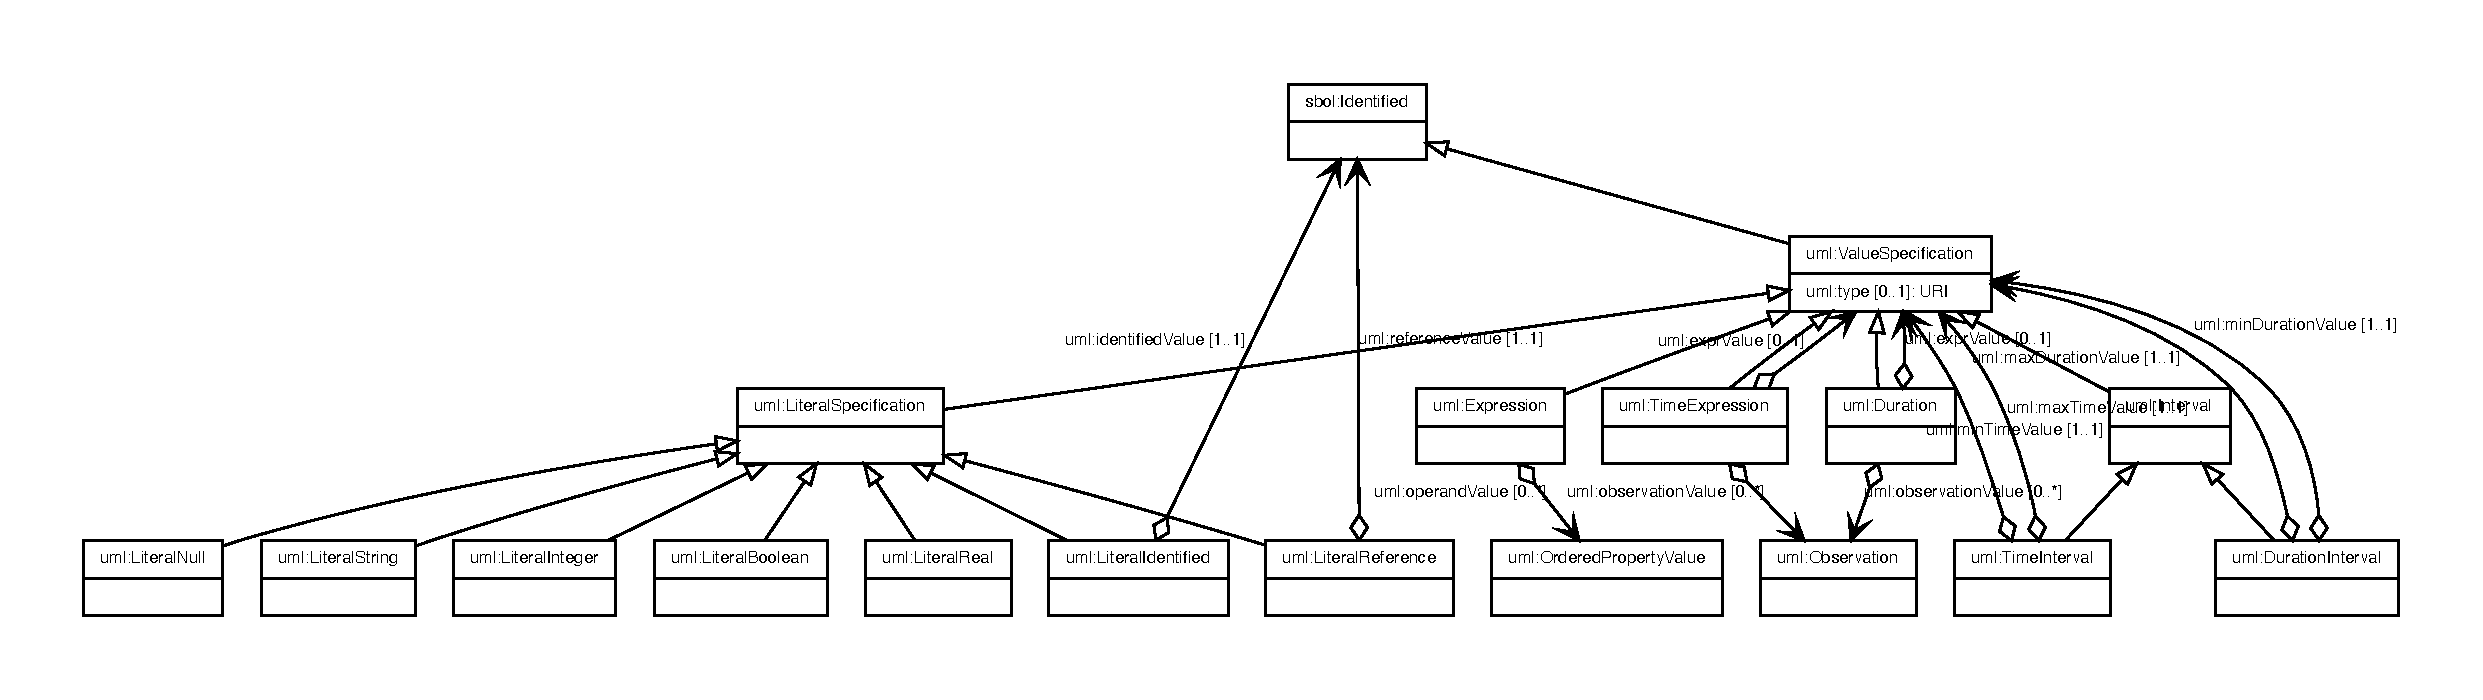
\includegraphics[width=1.0\textwidth]{uml_classes/ValueSpecification_abstraction_hierarchy.pdf}%
\caption{ValueSpecification}%
\label{fig:ValueSpecification}%
\end{figure}

%
The \uml{ValueSpecification} class is shown in \ref{fig:ValueSpecification}. It is derived from \sbol{Identified} and includes the following specializations: \uml{LiteralSpecification}, \uml{Expression}, \uml{TimeExpression}, \uml{Duration}, \uml{Interval}. %
This class includes the following properties: \uml{type}. %
\begin{itemize}%
\item%
The \uml{type} property is OPTIONAL and has a singleton value of type URISpecifies a set of Type instances constraining the allowed values. See UML 2.5.1 specification section 7.5.%
\end{itemize}%
\subsubsection{LiteralSpecification}%
\label{sec:uml:LiteralSpecification}%
A \uml{LiteralSpecification} identifies a literal constant being modeled. See UML 2.5.1 specification section 8.2.%
\newline%
\linebreak%
The \uml{LiteralSpecification} class is shown in \ref{fig:ValueSpecification}. It is derived from \uml{ValueSpecification} and includes the following specializations: \uml{LiteralNull}, \uml{LiteralString}, \uml{LiteralInteger}, \uml{LiteralBoolean}, \uml{LiteralReal}, \uml{LiteralIdentified}, \uml{LiteralReference}. %
%
\paragraph{LiteralNull}%
\label{sec:uml:LiteralNull}%
A \uml{LiteralNull} specifies the lack of a value. See UML 2.5.1 specification section 8.2.%
\newline%
\linebreak%
The \uml{LiteralNull} class is shown in \ref{fig:ValueSpecification}. It is derived from \uml{LiteralSpecification}.%
%
\paragraph{LiteralString}%
\label{sec:uml:LiteralString}%
A \uml{LiteralSpecification} identifies a literal constant being modeled. See UML 2.5.1 specification section 8.2.%
\newline%
\linebreak%
The \uml{LiteralString} class is shown in \ref{fig:ValueSpecification}. It is derived from \uml{LiteralSpecification}.%
This class includes the following properties: \uml{stringValue}. %
\begin{itemize}%
\item%
The \uml{stringValue} property is REQUIRED and has a singleton value of type stringThe specified String value.%
\end{itemize}%
\paragraph{LiteralInteger}%
\label{sec:uml:LiteralInteger}%
A \uml{LiteralInteger} is a specification of an Integer value. See UML 2.5.1 specification section 8.2.%
\newline%
\linebreak%
The \uml{LiteralInteger} class is shown in \ref{fig:ValueSpecification}. It is derived from \uml{LiteralSpecification}.%
This class includes the following properties: \uml{integerValue}. %
\begin{itemize}%
\item%
The \uml{integerValue} property is REQUIRED and has a singleton value of type integerThe specified Integer value.%
\end{itemize}%
\paragraph{LiteralBoolean}%
\label{sec:uml:LiteralBoolean}%
A \uml{LiteralBoolean} is a specification of a Boolean value. See UML 2.5.1 specification section 8.2.%
\newline%
\linebreak%
The \uml{LiteralBoolean} class is shown in \ref{fig:ValueSpecification}. It is derived from \uml{LiteralSpecification}.%
This class includes the following properties: \uml{booleanValue}. %
\begin{itemize}%
\item%
The \uml{booleanValue} property is REQUIRED and has a singleton value of type booleanThe specified Boolean value.%
\end{itemize}%
\paragraph{LiteralReal}%
\label{sec:uml:LiteralReal}%
A \uml{LiteralReal} is a specification of a Real value. See UML 2.5.1 specification section 8.2.%
\newline%
\linebreak%
The \uml{LiteralReal} class is shown in \ref{fig:ValueSpecification}. It is derived from \uml{LiteralSpecification}.%
This class includes the following properties: \uml{realValue}. %
\begin{itemize}%
\item%
The \uml{realValue} property is REQUIRED and has a singleton value of type floatThe specified Real value.%
\end{itemize}%
\paragraph{LiteralIdentified}%
\label{sec:uml:LiteralIdentified}%
A \uml{LiteralIdentified} is used for linking SBOL objects as a child object to UML objects.%
\newline%
\linebreak%
The \uml{LiteralIdentified} class is shown in \ref{fig:ValueSpecification}. It is derived from \uml{LiteralSpecification}.%
This class includes the following properties: \uml{identifiedValue}. %
\begin{itemize}%
\item%
The \uml{identifiedValue} property is REQUIRED and contains a URI reference to an associated object of type IdentifiedThe embedded SBOL object%
\end{itemize}%
\paragraph{LiteralReference}%
\label{sec:uml:LiteralReference}%
A \uml{LiteralReference} is used for embedding SBOL objects as a reference.%
\newline%
\linebreak%
The \uml{LiteralReference} class is shown in \ref{fig:ValueSpecification}. It is derived from \uml{LiteralSpecification}.%
This class includes the following properties: \uml{referenceValue}. %
\begin{itemize}%
\item%
The \uml{referenceValue} property is REQUIRED and contains a URI reference to an associated object of type IdentifiedThe referenced SBOL object.%
\end{itemize}%
\subsubsection{Expression}%
\label{sec:uml:Expression}%
An \uml{Expression} represents a node in an expression tree, which may be non-terminal or terminal. It defines a symbol, and has a possibly empty sequence of operands that are ValueSpecifications. See UML 2.5.1 specification section 8.6.5.1.%
\newline%
\linebreak%
The \uml{Expression} class is shown in \ref{fig:ValueSpecification}. It is derived from \uml{ValueSpecification}.%
This class includes the following properties: \uml{isOrdered}, \uml{symbolValue}, \uml{operandValue}. %
\begin{itemize}%
\item%
The \uml{operandValue} property is OPTIONAL and contains URI references to associated objects of type OrderedPropertyValueSpecifies a sequence of operand ValueSpecifications.%
\item%
The \uml{isOrdered} property is REQUIRED and has a singleton value of type booleanFor MultiplicityElement abstract class; UML 2.5.1 specification section 7.5%
\item%
The \uml{symbolValue} property is OPTIONAL and has a singleton value of type stringThe symbol associated with this node in the expression tree.%
\end{itemize}%
\subsubsection{TimeExpression}%
\label{sec:uml:TimeExpression}%
A \uml{TimeExpression} is a \uml{ValueSpecification} that represents a time value.%
\newline%
\linebreak%
The \uml{TimeExpression} class is shown in \ref{fig:ValueSpecification}. It is derived from \uml{ValueSpecification}.%
This class includes the following properties: \uml{observationValue}, \uml{exprValue}. %
\begin{itemize}%
\item%
The \uml{observationValue} property is OPTIONAL and contains URI references to associated objects of type ObservationRefers to the Observations that are involved in the computation of the Duration value.%
\item%
The \uml{exprValue} property is OPTIONAL and contains a URI reference to an associated object of type ValueSpecificationA ValueSpecification that evaluates to the value of the Duration.%
\end{itemize}%
\subsubsection{Duration}%
\label{sec:uml:Duration}%
A \uml{Duration} is a \uml{ValueSpecification} that specifies the temporal distance between two time instants.%
\newline%
\linebreak%
The \uml{Duration} class is shown in \ref{fig:ValueSpecification}. It is derived from \uml{ValueSpecification}.%
This class includes the following properties: \uml{observationValue}, \uml{exprValue}. %
\begin{itemize}%
\item%
The \uml{observationValue} property is OPTIONAL and contains URI references to associated objects of type ObservationRefers to the Observations that are involved in the computation of the Duration value.%
\item%
The \uml{exprValue} property is OPTIONAL and contains a URI reference to an associated object of type ValueSpecificationA ValueSpecification that evaluates to the value of the Duration.%
\end{itemize}%
\subsubsection{Interval}%
\label{sec:uml:Interval}%
An \uml{Interval} defines the range between two ValueSpecifications.%
\newline%
\linebreak%
The \uml{Interval} class is shown in \ref{fig:ValueSpecification}. It is derived from \uml{ValueSpecification} and includes the following specializations: \uml{TimeInterval}, \uml{DurationInterval}. %
%
\paragraph{TimeInterval}%
\label{sec:uml:TimeInterval}%
A \uml{TimeInterval} defines the range between two TimeExpressions.%
\newline%
\linebreak%
The \uml{TimeInterval} class is shown in \ref{fig:ValueSpecification}. It is derived from \uml{Interval}.%
This class includes the following properties: \uml{minTimeValue}, \uml{maxTimeValue}. %
\begin{itemize}%
\item%
The \uml{minTimeValue} property is REQUIRED and contains a URI reference to an associated object of type ValueSpecificationRefers to the TimeExpression denoting the minimum value of the range.%
\item%
The \uml{maxTimeValue} property is REQUIRED and contains a URI reference to an associated object of type ValueSpecificationRefers to the TimeExpression denoting the maximum value of the range.%
\end{itemize}%
\paragraph{DurationInterval}%
\label{sec:uml:DurationInterval}%
A \uml{DurationInterval} defines the range between two Durations.%
\newline%
\linebreak%
The \uml{DurationInterval} class is shown in \ref{fig:ValueSpecification}. It is derived from \uml{Interval}.%
This class includes the following properties: \uml{minDurationValue}, \uml{maxDurationValue}. %
\begin{itemize}%
\item%
The \uml{minDurationValue} property is REQUIRED and contains a URI reference to an associated object of type ValueSpecificationRefers to the Duration denoting the minimum value of the range.%
\item%
The \uml{maxDurationValue} property is REQUIRED and contains a URI reference to an associated object of type ValueSpecificationRefers to the Duration denoting the maximum value of the range.%
\end{itemize}%
\subsection{Observation}%
\label{sec:uml:Observation}%
Observation specifies a value determined by observing an event or events that occur relative to other model entities.%
\newline%
\linebreak%


\begin{figure}[h!]%
\centering%
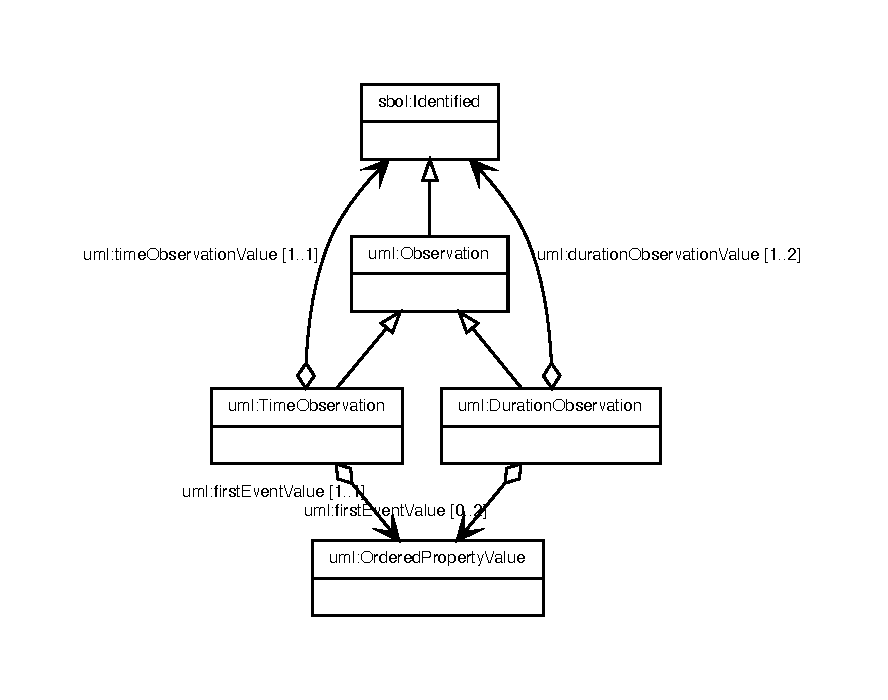
\includegraphics[width=0.634468085106383\textwidth]{uml_classes/Observation_abstraction_hierarchy.pdf}%
\caption{Observation}%
\label{fig:Observation}%
\end{figure}

%
The \uml{Observation} class is shown in \ref{fig:Observation}. It is derived from \sbol{Identified} and includes the following specializations: \uml{TimeObservation}, \uml{DurationObservation}. %
%
\subsubsection{TimeObservation}%
\label{sec:uml:TimeObservation}%
A \uml{TimeObservation} is a reference to a time instant during an execution. It points out which entity in the model to observe and whether the observation is when this entity is entered or when it is exited.%
\newline%
\linebreak%
The \uml{TimeObservation} class is shown in \ref{fig:Observation}. It is derived from \uml{Observation}.%
This class includes the following properties: \uml{timeObservationValue}, \uml{firstEventValue}. %
\begin{itemize}%
\item%
The \uml{timeObservationValue} property is REQUIRED and contains a URI reference to an associated object of type IdentifiedThe TimeObservation is determined by the entering or exiting of the event during execution.%
\item%
The \uml{firstEventValue} property is REQUIRED and contains a URI reference to an associated object of type OrderedPropertyValueThe value of firstEvent[i] is related to event[i] (where i is 1 or 2). If firstEvent[i] is true, then the correspondingobservation event is the first time instant the execution enters event[i]. If firstEvent[i] is false, then the corresponding observation event is the time instant the execution exits event[i].%
\end{itemize}%
\subsubsection{DurationObservation}%
\label{sec:uml:DurationObservation}%
A \uml{DurationObservation} is a reference to a duration during an execution. It points out the entities in the model to observe and whether the observations are when these entities are entered or exited.%
\newline%
\linebreak%
The \uml{DurationObservation} class is shown in \ref{fig:Observation}. It is derived from \uml{Observation}.%
This class includes the following properties: \uml{durationObservationValue}, \uml{firstEventValue}. %
\begin{itemize}%
\item%
The \uml{durationObservationValue} property is REQUIRED and contains URI references to associated objects of type IdentifiedThe DurationObservation is determined as the duration between the entering or exiting of a single event during execution, or the entering/exiting of one event and the entering/exiting of a second.%
\item%
The \uml{firstEventValue} property is OPTIONAL and contains URI references to associated objects of type OrderedPropertyValueThe value of firstEvent[i] is related to event[i] (where i is 1 or 2). If firstEvent[i] is true, then the correspondingobservation event is the first time instant the execution enters event[i]. If firstEvent[i] is false, then the corresponding observation event is the time instant the execution exits event[i].%
\end{itemize}%
\subsection{Constraint}%
\label{sec:uml:Constraint}%
A \sbol{Constraint} is a condition or restriction expressed in natural language text or in a machine readable language. See UML 2.5.1 specification section 7.6.%
\newline%
\linebreak%


\begin{figure}[h!]%
\centering%
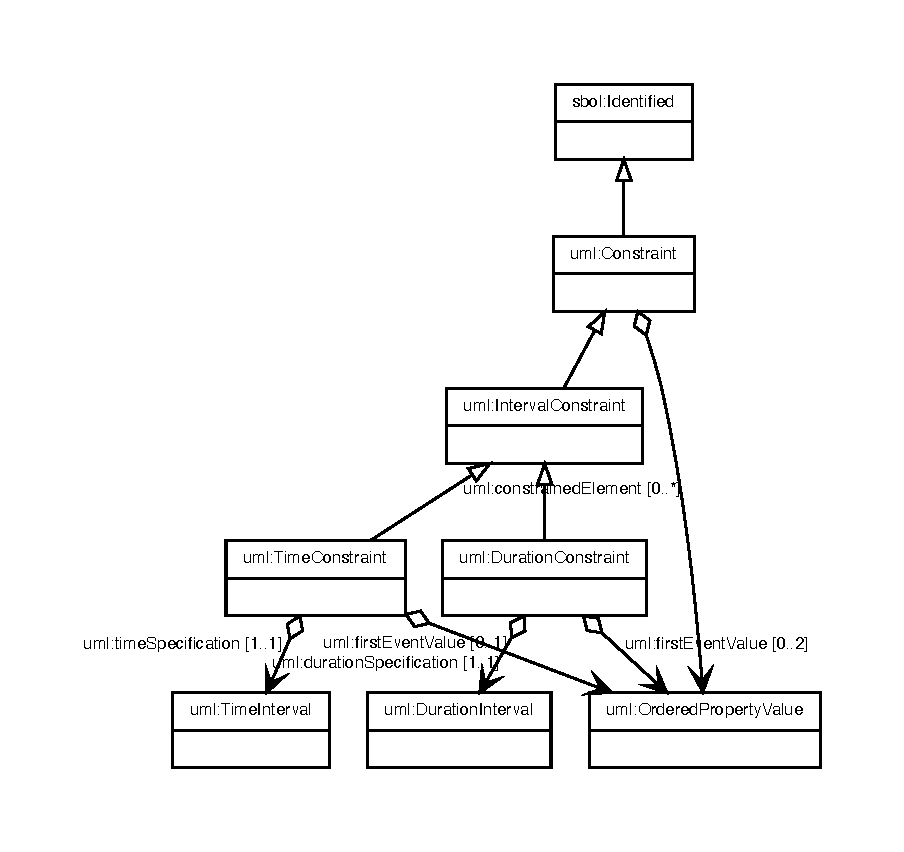
\includegraphics[width=0.7178723404255319\textwidth]{uml_classes/Constraint_abstraction_hierarchy.pdf}%
\caption{Constraint}%
\label{fig:Constraint}%
\end{figure}

%
The \uml{Constraint} class is shown in \ref{fig:Constraint}. It is derived from \sbol{Identified} and includes the following specializations: \uml{IntervalConstraint}. %
This class includes the following properties: \uml{constrainedElement}. %
\begin{itemize}%
\item%
The \uml{constrainedElement} property is OPTIONAL and contains URI references to associated objects of type OrderedPropertyValueThe OrderedPropertyValue referenced by this Constraint.%
\end{itemize}%
\subsubsection{IntervalConstraint}%
\label{sec:uml:IntervalConstraint}%
An \uml{IntervalConstraint} is a \sbol{Constraint} that is specified by an \uml{Interval}.%
\newline%
\linebreak%
The \uml{IntervalConstraint} class is shown in \ref{fig:Constraint}. It is derived from \uml{Constraint} and includes the following specializations: \uml{TimeConstraint}, \uml{DurationConstraint}. %
%
\paragraph{TimeConstraint}%
\label{sec:uml:TimeConstraint}%
A \uml{TimeConstraint} is a \sbol{Constraint} that refers to a \uml{TimeInterval}.%
\newline%
\linebreak%
The \uml{TimeConstraint} class is shown in \ref{fig:Constraint}. It is derived from \uml{IntervalConstraint}.%
This class includes the following properties: \uml{timeSpecification}, \uml{firstEventValue}. %
\begin{itemize}%
\item%
The \uml{timeSpecification} property is REQUIRED and contains a URI reference to an associated object of type TimeIntervalTheTimeInterval constraining the duration.%
\item%
The \uml{firstEventValue} property is OPTIONAL and contains a URI reference to an associated object of type OrderedPropertyValueThe value of firstEvent[i] is related to event[i] (where i is 1 or 2). If firstEvent[i] is true, then the correspondingobservation event is the first time instant the execution enters event[i]. If firstEvent[i] is false, then the corresponding observation event is the time instant the execution exits event[i].%
\end{itemize}%
\paragraph{DurationConstraint}%
\label{sec:uml:DurationConstraint}%
A \uml{DurationConstraint} is a \sbol{Constraint} that refers to a \uml{DurationInterval}.%
\newline%
\linebreak%
The \uml{DurationConstraint} class is shown in \ref{fig:Constraint}. It is derived from \uml{IntervalConstraint}.%
This class includes the following properties: \uml{durationSpecification}, \uml{firstEventValue}. %
\begin{itemize}%
\item%
The \uml{durationSpecification} property is REQUIRED and contains a URI reference to an associated object of type DurationIntervalThe DurationInterval constraining the duration.%
\item%
The \uml{firstEventValue} property is OPTIONAL and contains URI references to associated objects of type OrderedPropertyValueThe value of firstEvent[i] is related to event[i] (where i is 1 or 2). If firstEvent[i] is true, then the correspondingobservation event is the first time instant the execution enters event[i]. If firstEvent[i] is false, then the corresponding observation event is the time instant the execution exits event[i].%
\end{itemize}%
\subsection{Parameter}%
\label{sec:uml:Parameter}%
A \uml{Parameter} is a specification of an argument used to pass information into or out of an invocation of a \uml{Behavior}. See UML 2.5.1 specification section 9.4.%
\newline%
\linebreak%


\begin{figure}[h!]%
\centering%
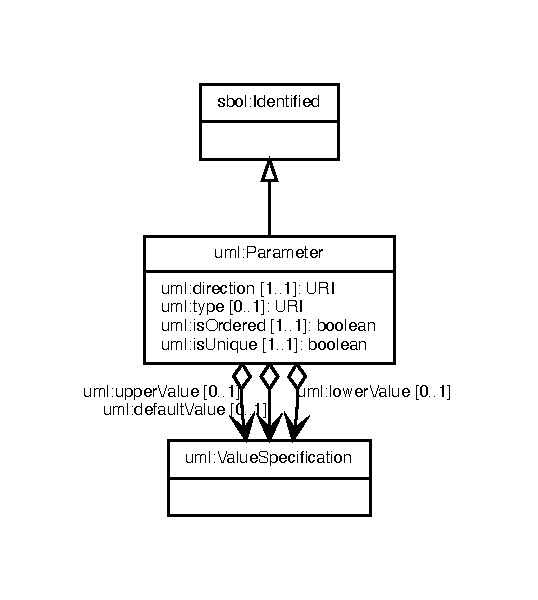
\includegraphics[width=0.3842553191489362\textwidth]{uml_classes/Parameter_abstraction_hierarchy.pdf}%
\caption{Parameter}%
\label{fig:Parameter}%
\end{figure}

%
The \uml{Parameter} class is shown in \ref{fig:Parameter}. It is derived from \sbol{Identified}.%
This class includes the following properties: \uml{direction}, \uml{type}, \uml{isOrdered}, \uml{isUnique}, \uml{upperValue}, \uml{defaultValue}, \uml{lowerValue}. %
\begin{itemize}%
\item%
The \uml{upperValue} property is OPTIONAL and contains a URI reference to an associated object of type ValueSpecificationFor MultiplicityElement abstract class; UML 2.5.1 specification section 7.5%
\item%
The \uml{defaultValue} property is OPTIONAL and contains a URI reference to an associated object of type ValueSpecificationA ValueSpecification that represents a value to be used when no argument is supplied for the Parameter.%
\item%
The \uml{lowerValue} property is OPTIONAL and contains a URI reference to an associated object of type ValueSpecificationFor MultiplicityElement abstract class; UML 2.5.1 specification section 7.5%
\item%
The \uml{direction} property is REQUIRED and has a singleton value of type URIIndicates whether a parameter is being sent into or out of a behavioral element.%
\item%
The \uml{type} property is OPTIONAL and has a singleton value of type URISpecifies a set of Type instances constraining the allowed values. See UML 2.5.1 specification section 7.5.%
\item%
The \uml{isOrdered} property is REQUIRED and has a singleton value of type booleanFor MultiplicityElement abstract class; UML 2.5.1 specification section 7.5%
\item%
The \uml{isUnique} property is REQUIRED and has a singleton value of type booleanFor MultiplicityElement abstract class; UML 2.5.1 specification section 7.5%
\end{itemize}%
\subsection{Behavior}%
\label{sec:uml:Behavior}%
Behavior is an abstract specification of how a state changes over time. This specification may be a prospective definition of a protocol or a capture of an execution trace. See UML 2.5.1 specification section 13.2.%
\newline%
\linebreak%


\begin{figure}[h!]%
\centering%
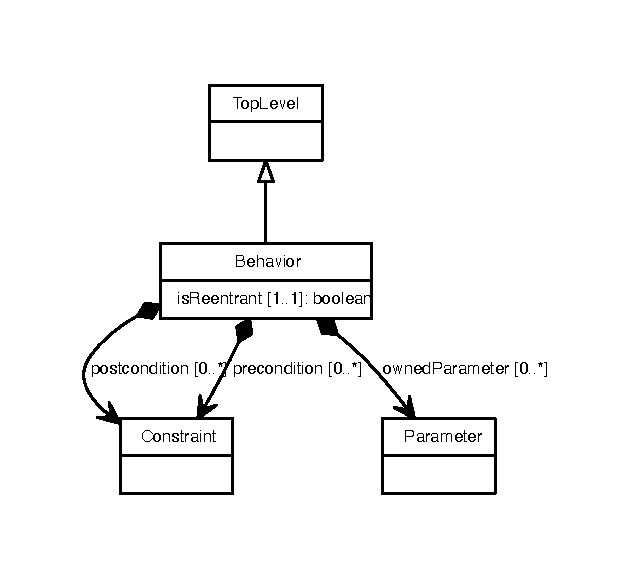
\includegraphics[width=0.6448936170212766\textwidth]{uml_classes/Behavior_abstraction_hierarchy.pdf}%
\caption{Behavior}%
\label{fig:Behavior}%
\end{figure}

%
The \uml{Behavior} class is shown in \ref{fig:Behavior}. It is derived from \sbol{TopLevel} and includes the following specializations: \uml{Activity}. %
This class includes the following properties: \uml{ownedParameter}, \uml{postcondition}, \uml{precondition}. %
\begin{itemize}%
\item%
The \uml{ownedParameter} property is OPTIONAL and contains URI references to associated objects of type OrderedPropertyValue a list of Parameters to the Behavior which describes the order and type of arguments that can be given when the Behavior is invoked and of the values which will be returned when the Behavior completes its execution.%
\item%
The \uml{postcondition} property is OPTIONAL and contains URI references to associated objects of type ConstraintAn optional set of Constraints specifying what is fulfilled after the execution of the Behavior is completed, if its precondition was fulfilled before its invocation.%
\item%
The \uml{precondition} property is OPTIONAL and contains URI references to associated objects of type ConstraintAn optional set of Constraints specifying what must be fulfilled before the Behavior is invoked.%
\end{itemize}%
\subsubsection{Activity}%
\label{sec:uml:Activity}%
An \prov{Activity} coordinates and groups steps in a protocol or workflow. See UML 2.5.1 specification section 15.%
\newline%
\linebreak%
The \uml{Activity} class is shown in \ref{fig:Behavior}. It is derived from \uml{Behavior}.%
This class includes the following properties: \uml{edge}, \uml{node}. %
\begin{itemize}%
\item%
The \uml{edge} property is OPTIONAL and contains URI references to associated objects of type ActivityEdgeActivityEdges expressing flow between the nodes of the Activity.%
\item%
The \uml{node} property is OPTIONAL and contains URI references to associated objects of type ActivityNodeActivityNodes coordinated by the Activity.%
\end{itemize}%
\subsection{OrderedPropertyValue}%
\label{sec:uml:OrderedPropertyValue}%


\begin{figure}[h!]%
\centering%
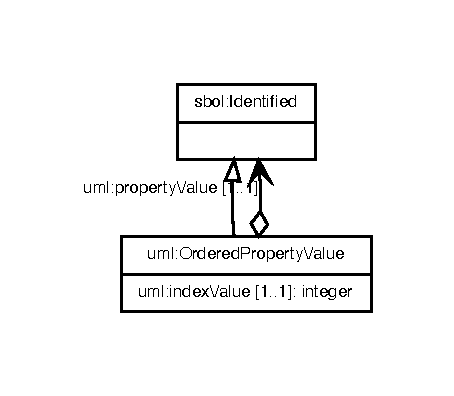
\includegraphics[width=0.32468085106382977\textwidth]{uml_classes/OrderedPropertyValue_abstraction_hierarchy.pdf}%
\caption{OrderedPropertyValue}%
\label{fig:OrderedPropertyValue}%
\end{figure}

%
The \uml{OrderedPropertyValue} class is shown in \ref{fig:OrderedPropertyValue}. It is derived from \sbol{Identified}.%
This class includes the following properties: \uml{indexValue}, \uml{propertyValue}. %
\begin{itemize}%
\item%
The \uml{propertyValue} property is REQUIRED and contains a URI reference to an associated object of type Identified%
\item%
The \uml{indexValue} property is REQUIRED and has a singleton value of type integer%
\end{itemize}%
\subsection{ActivityNode}%
\label{sec:uml:ActivityNode}%
ActivityNode is an abstract class for points in the flow of an \prov{Activity} connected by ActivityEdges. See UML 2.5.1 specification section 15.2.%
\newline%
\linebreak%


\begin{figure}[h!]%
\centering%
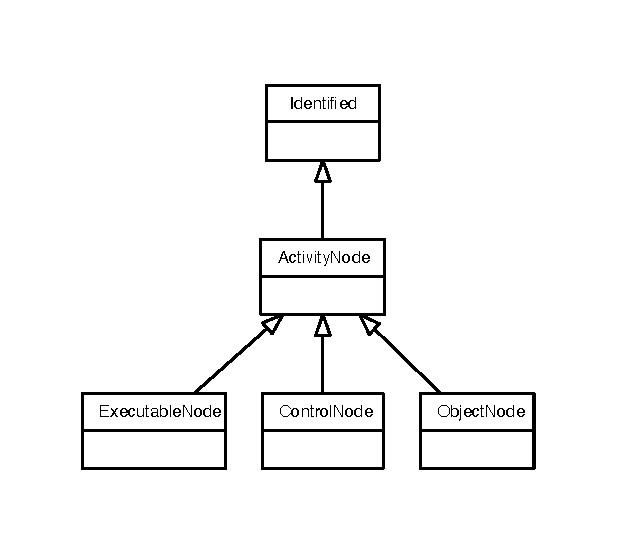
\includegraphics[width=1.0\textwidth]{uml_classes/ActivityNode_abstraction_hierarchy.pdf}%
\caption{ActivityNode}%
\label{fig:ActivityNode}%
\end{figure}

%
The \uml{ActivityNode} class is shown in \ref{fig:ActivityNode}. It is derived from \sbol{Identified} and includes the following specializations: \uml{ControlNode}, \uml{ObjectNode}, \uml{ExecutableNode}. %
%
\subsubsection{ControlNode}%
\label{sec:uml:ControlNode}%
A \uml{ControlNode} is a kind of \uml{ActivityNode} used to manage the flow of tokens between other nodes in an \prov{Activity}. It can manage branching and merging of workflows and the implementation of logic for flow control. See UML 2.5.1 specification section 15.3.%
\newline%
\linebreak%
The \uml{ControlNode} class is shown in \ref{fig:ActivityNode}. It is derived from \uml{ActivityNode} and includes the following specializations: \uml{InitialNode}, \uml{FinalNode}, \uml{ForkNode}, \uml{JoinNode}, \uml{MergeNode}, \uml{DecisionNode}. %
%
\paragraph{InitialNode}%
\label{sec:uml:InitialNode}%
An \uml{InitialNode} acts as a starting point for executing an \prov{Activity}. An \prov{Activity} may have more than \sbol{one} InitialNodes that start multiple concurrent control flows. See UML 2.5.1 specification section 15.3.%
\newline%
\linebreak%
The \uml{InitialNode} class is shown in \ref{fig:ActivityNode}. It is derived from \uml{ControlNode}.%
%
\paragraph{FinalNode}%
\label{sec:uml:FinalNode}%
A \uml{FinalNode} is a \uml{ControlNode} at which a flow in an \prov{Activity} stops. A \uml{FinalNode} shall not have outgoing ActivityEdges. See UML 2.5.1 specification section 15.3.%
\newline%
\linebreak%
The \uml{FinalNode} class is shown in \ref{fig:ActivityNode}. It is derived from \uml{ControlNode} and includes the following specializations: \uml{FlowFinalNode}. %
%
\subparagraph{FlowFinalNode}%
\label{sec:uml:FlowFinalNode}%
A \uml{FlowFinalNode} is a \uml{FinalNode} that terminates a flow. All tokens accepted by a \uml{FlowFinalNode} are destroyed. This has no effect on other flows in the \prov{Activity}. See UML 2.5.1 specification section 15.3.%
\newline%
\linebreak%
The \uml{FlowFinalNode} class is shown in \ref{fig:ActivityNode}. It is derived from \uml{FinalNode}.%
%
\paragraph{ForkNode}%
\label{sec:uml:ForkNode}%
A \uml{ForkNode} is a \uml{ControlNode} that splits a flow into multiple concurrent flows. A \uml{ForkNode} shall have exactly \sbol{one} incoming \uml{ActivityEdge}, though it may have multiple outgoing ActivityEdges. See UML 2.5.1 specification section 15.3.%
\newline%
\linebreak%
The \uml{ForkNode} class is shown in \ref{fig:ActivityNode}. It is derived from \uml{ControlNode}.%
%
\paragraph{JoinNode}%
\label{sec:uml:JoinNode}%
A \uml{JoinNode} is a \uml{ControlNode} that synchronizes multiple flows. A \uml{JoinNode} shall have exactly \sbol{one} outgoing \uml{ActivityEdge} but may have multiple incoming ActivityEdges. See UML 2.5.1 specification section 15.3.%
\newline%
\linebreak%
The \uml{JoinNode} class is shown in \ref{fig:ActivityNode}. It is derived from \uml{ControlNode}.%
%
\paragraph{MergeNode}%
\label{sec:uml:MergeNode}%
A \uml{MergeNode} is a control node that brings together multiple flows without synchronization. A \uml{MergeNode} shall have exactly \sbol{one} outgoing \uml{ActivityEdge} but may have multiple incoming ActivityEdges. See UML 2.5.1 specification section 15.3.%
\newline%
\linebreak%
The \uml{MergeNode} class is shown in \ref{fig:ActivityNode}. It is derived from \uml{ControlNode}.%
%
\paragraph{DecisionNode}%
\label{sec:uml:DecisionNode}%
A \uml{DecisionNode} is a \uml{ControlNode} that chooses between outgoing flows. A \uml{DecisionNode} shall have at least \sbol{one} and at most two incoming ActivityEdges, and at least \sbol{one} outgoing \uml{ActivityEdge}. See UML 2.5.1 specification section 15.3.%
\newline%
\linebreak%
The \uml{DecisionNode} class is shown in \ref{fig:ActivityNode}. It is derived from \uml{ControlNode}.%
This class includes the following properties: \uml{decisionInput}, \uml{decisionInputFlow}. %
\begin{itemize}%
\item%
The \uml{decisionInput} property is OPTIONAL and contains a URI reference to an associated object of type BehaviorA Behavior that is executed to provide an input to guard ValueSpecifications on ActivityEdges outgoing from the DecisionNode.%
\item%
The \uml{decisionInputFlow} property is OPTIONAL and contains a URI reference to an associated object of type ObjectFlowAn additional ActivityEdge incoming to the DecisionNode that provides a decision input value for the guards ValueSpecifications on ActivityEdges outgoing from the DecisionNode.%
\end{itemize}%
\subsubsection{ObjectNode}%
\label{sec:uml:ObjectNode}%
An \uml{ObjectNode} is a kind of \uml{ActivityNode} used to hold value-containing object tokens during the course of the execution of an \prov{Activity}. See UML 2.5.1 specification section 15.4.%
\newline%
\linebreak%
The \uml{ObjectNode} class is shown in \ref{fig:ActivityNode}. It is derived from \uml{ActivityNode} and includes the following specializations: \uml{ActivityParameterNode}, \uml{Pin}. %
This class includes the following properties: \uml{type}. %
\begin{itemize}%
\item%
The \uml{type} property is OPTIONAL and has a singleton value of type URISpecifies a set of Type instances constraining the allowed values. See UML 2.5.1 specification section 7.5.%
\end{itemize}%
\paragraph{ActivityParameterNode}%
\label{sec:uml:ActivityParameterNode}%
An \uml{ActivityParameterNode} is an \uml{ObjectNode} for accepting values from the input Parameters or providing values to the output Parameters of an \prov{Activity}. UML 2.5.1 specification section 15.4.%
\newline%
\linebreak%
The \uml{ActivityParameterNode} class is shown in \ref{fig:ActivityNode}. It is derived from \uml{ObjectNode}.%
This class includes the following properties: \uml{parameter}. %
\begin{itemize}%
\item%
The \uml{parameter} property is REQUIRED and contains a URI reference to an associated object of type ParameterThe Parameter for which the ActivityParameterNode will be accepting or providing values.%
\end{itemize}%
\paragraph{Pin}%
\label{sec:uml:Pin}%
A \uml{Pin} is an \uml{ObjectNode} and MultiplicityElement that provides input values to an \uml{Action} or accepts output values from an \uml{Action}. See UML 2.5.1 specification section 16.2.%
\newline%
\linebreak%
The \uml{Pin} class is shown in \ref{fig:ActivityNode}. It is derived from \uml{ObjectNode} and includes the following specializations: \uml{InputPin}, \uml{OutputPin}. %
This class includes the following properties: \uml{isOrdered}, \uml{isUnique}, \uml{upperValue}, \uml{lowerValue}. %
\begin{itemize}%
\item%
The \uml{upperValue} property is OPTIONAL and contains a URI reference to an associated object of type ValueSpecificationFor MultiplicityElement abstract class; UML 2.5.1 specification section 7.5%
\item%
The \uml{lowerValue} property is OPTIONAL and contains a URI reference to an associated object of type ValueSpecificationFor MultiplicityElement abstract class; UML 2.5.1 specification section 7.5%
\item%
The \uml{isOrdered} property is REQUIRED and has a singleton value of type booleanFor MultiplicityElement abstract class; UML 2.5.1 specification section 7.5%
\item%
The \uml{isUnique} property is REQUIRED and has a singleton value of type booleanFor MultiplicityElement abstract class; UML 2.5.1 specification section 7.5%
\end{itemize}%
\subparagraph{InputPin}%
\label{sec:uml:InputPin}%
An \uml{InputPin} is a \uml{Pin} that holds input values to be consumed by an \uml{Action}. See UML 2.5.1 specification section 16.2.%
\newline%
\linebreak%
The \uml{InputPin} class is shown in \ref{fig:ActivityNode}. It is derived from \uml{Pin} and includes the following specializations: \uml{ValuePin}. %
%
\subparagraph{ValuePin}%
\label{sec:uml:ValuePin}%
A \uml{ValuePin} is an \uml{InputPin} that provides a value by evaluating a \uml{ValueSpecification}. See UML 2.5.1 specification section 16.2.%
\newline%
\linebreak%
The \uml{ValuePin} class is shown in \ref{fig:ActivityNode}. It is derived from \uml{InputPin}.%
This class includes the following properties: \uml{value}. %
\begin{itemize}%
\item%
The \uml{value} property is REQUIRED and contains a URI reference to an associated object of type ValueSpecificationThe ValueSpecification that is evaluated to obtain the value that the ValuePin will provide.%
\end{itemize}%
\subparagraph{OutputPin}%
\label{sec:uml:OutputPin}%
An \uml{OutputPin} is a \uml{Pin} that holds output values produced by an \uml{Action}. See UML 2.5.1 specification section 16.2.%
\newline%
\linebreak%
The \uml{OutputPin} class is shown in \ref{fig:ActivityNode}. It is derived from \uml{Pin}.%
%
\subsubsection{ExecutableNode}%
\label{sec:uml:ExecutableNode}%
An \uml{ExecutableNode} is an abstract class for ActivityNodes whose execution may be controlled using ControlFlows and to which ExceptionHandlers may be attached. See UML 2.5.1 specification section 15.5.%
\newline%
\linebreak%
The \uml{ExecutableNode} class is shown in \ref{fig:ActivityNode}. It is derived from \uml{ActivityNode} and includes the following specializations: \uml{Action}. %
%
\paragraph{Action}%
\label{sec:uml:Action}%
An \uml{Action} is the fundamental unit of executable functionality. The execution of an \uml{Action} represents some transformation or processing in the modeled system. Actions provide the ExecutableNodes within Activities and may also be used within Interactions. See UML 2.5.1 specification section 16.%
\newline%
\linebreak%
The \uml{Action} class is shown in \ref{fig:ActivityNode}. It is derived from \uml{ExecutableNode} and includes the following specializations: \uml{InvocationAction}. %
This class includes the following properties: \uml{output}, \uml{input}. %
\begin{itemize}%
\item%
The \uml{output} property is OPTIONAL and contains URI references to associated objects of type OutputPinThe ordered set of OutputPins representing outputs from the Action.%
\item%
The \uml{input} property is OPTIONAL and contains URI references to associated objects of type InputPinThe ordered set of InputPins representing the inputs to the Action.%
\end{itemize}%
\subparagraph{InvocationAction}%
\label{sec:uml:InvocationAction}%
UML 2.5.1 specification section 16.3%
\newline%
\linebreak%
The \uml{InvocationAction} class is shown in \ref{fig:ActivityNode}. It is derived from \uml{Action} and includes the following specializations: \uml{CallAction}. %
%
\subparagraph{CallAction}%
\label{sec:uml:CallAction}%
A \uml{CallAction} is an abstract class for Actions that invoke a \uml{Behavior} with given argument values and (if the invocation is synchronous) receive reply values. See UML 2.5.1 specification section 16.3.%
\newline%
\linebreak%
The \uml{CallAction} class is shown in \ref{fig:ActivityNode}. It is derived from \uml{InvocationAction} and includes the following specializations: \uml{CallBehaviorAction}. %
%
\subparagraph{CallBehaviorAction}%
\label{sec:uml:CallBehaviorAction}%
A \uml{CallBehaviorAction} is a \uml{CallAction} that invokes a \uml{Behavior} directly. The argument values of the \uml{CallBehaviorAction} are passed on the input Parameters of the invoked \uml{Behavior}. UML 2.5.1 specification section 16.3%
\newline%
\linebreak%
The \uml{CallBehaviorAction} class is shown in \ref{fig:ActivityNode}. It is derived from \uml{CallAction}.%
This class includes the following properties: \uml{behavior}. %
\begin{itemize}%
\item%
The \uml{behavior} property is REQUIRED and contains a URI reference to an associated object of type BehaviorThe Behavior being invoked.%
\end{itemize}%
\subsection{ActivityEdge}%
\label{sec:uml:ActivityEdge}%
An \uml{ActivityEdge} is an abstract class for directed connections between two ActivityNodes. See UML 2.5.1 specification section 15.2.%
\newline%
\linebreak%


\begin{figure}[h!]%
\centering%
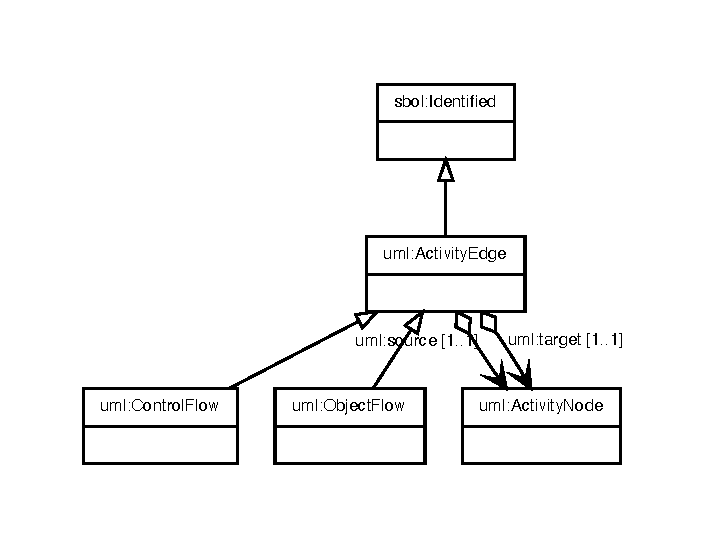
\includegraphics[width=0.5063829787234042\textwidth]{uml_classes/ActivityEdge_abstraction_hierarchy.pdf}%
\caption{ActivityEdge}%
\label{fig:ActivityEdge}%
\end{figure}

%
The \uml{ActivityEdge} class is shown in \ref{fig:ActivityEdge}. It is derived from \sbol{Identified} and includes the following specializations: \uml{ControlFlow}, \uml{ObjectFlow}. %
This class includes the following properties: \uml{source}, \uml{target}. %
\begin{itemize}%
\item%
The \uml{source} property is REQUIRED and contains a URI reference to an associated object of type ActivityNodeThe ActivityNode from which tokens are taken when they traverse the ActivityEdge.%
\item%
The \uml{target} property is REQUIRED and contains a URI reference to an associated object of type ActivityNodeThe ActivityNode to which tokens are put when they traverse the ActivityEdge.%
\end{itemize}%
\subsubsection{ControlFlow}%
\label{sec:uml:ControlFlow}%
A \uml{ControlFlow} is an \uml{ActivityEdge} traversed by control tokens or object tokens of control type, which are use to control the execution of ExecutableNodes. See UML 2.5.1 specification section 15.2.%
\newline%
\linebreak%
The \uml{ControlFlow} class is shown in \ref{fig:ActivityEdge}. It is derived from \uml{ActivityEdge}.%
%
\subsubsection{ObjectFlow}%
\label{sec:uml:ObjectFlow}%
An \uml{ObjectFlow} is an \uml{ActivityEdge} that is traversed by object tokens that may hold values. Object flows also support multicast/receive, token selection from object nodes, and transformation of tokens. See UML 2.5.1 specification section 15.2.%
\newline%
\linebreak%
The \uml{ObjectFlow} class is shown in \ref{fig:ActivityEdge}. It is derived from \uml{ActivityEdge}.%
%


\section{LabOP Data Model}
\label{sec:labop}
%
\normalsize%
\subsection{Protocol}%
\label{sec:labop:Protocol}%
A \labop{Protocol} describes how to carry out some form of laboratory or research process.
              For example, a \labop{Protocol} could describe DNA miniprep, Golden-Gate assembly, a cell culture experiment.
              At present this class adds no additional information over \uml{Activity}, but may in the future.%
\newline%
\linebreak%


\begin{figure}[h!]%
\centering%
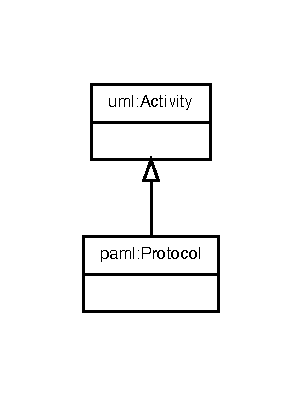
\includegraphics[width=0.21595744680851064\textwidth]{labop_classes/Protocol_abstraction_hierarchy.pdf}%
\caption{Protocol}%
\label{fig:Protocol}%
\end{figure}

%
The \labop{Protocol} class is shown in \ref{fig:Protocol}. It is derived from \uml{Activity}.%
%
\subsection{Primitive}%
\label{sec:labop:Primitive}%
A \labop{Primitive} describes a library function that acts as a basic ``building block'' for a \labop{Protocol}.
              For example, a \labop{Primitive} could describe pipetting, measuring absorbance in a plate reader, or centrifuging.
              At present this class adds no additional information over \uml{Behavior}, but may in the future.%
\newline%
\linebreak%


\begin{figure}[h!]%
\centering%
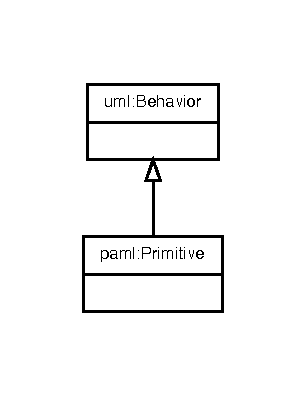
\includegraphics[width=0.21893617021276596\textwidth]{labop_classes/Primitive_abstraction_hierarchy.pdf}%
\caption{Primitive}%
\label{fig:Primitive}%
\end{figure}

%
The \labop{Primitive} class is shown in \ref{fig:Primitive}. It is derived from \uml{Behavior}.%
%
\subsection{BehaviorExecution}%
\label{sec:labop:BehaviorExecution}%
A \labop{BehaviorExecution} is a record of how a \labop{Protocol}, \labop{Primitive}, or other \uml{Behavior} was carried out.
        The execution of the behavior could be either real or simulated.

        In specifying a \labop{BehaviorExecution}, the prov:type field inherited from \prov{Activity} is used to indicate the
        \uml{Behavior} whose execution is being recorded. Precisely \sbol{one} value of prov:type MUST be a URI for a \uml{Behavior}.
        The prov:startedAtTime and prov:endedAtTime fields SHOULD be used to record timing information as this becomes
        available.
        Finally, the entity carrying out the execution SHOULD be recorded as a \prov{Agent} indicated using a
        \prov{Association}.

        Note that a \labop{BehaviorExecution} can be used to record both the state of an in-progress execution as well as an
        execution that has completed. As a \labop{BehaviorExecution} proceeds, all values of its properties are monotonic,
        i.e., they are only added to and never changed.

        TODO: need to changing completedNormally to allow indication of an in-progress BehaviorExecution
        TODO: Is there a good ontology for agent roles in association?%
\newline%
\linebreak%


\begin{figure}[h!]%
\centering%
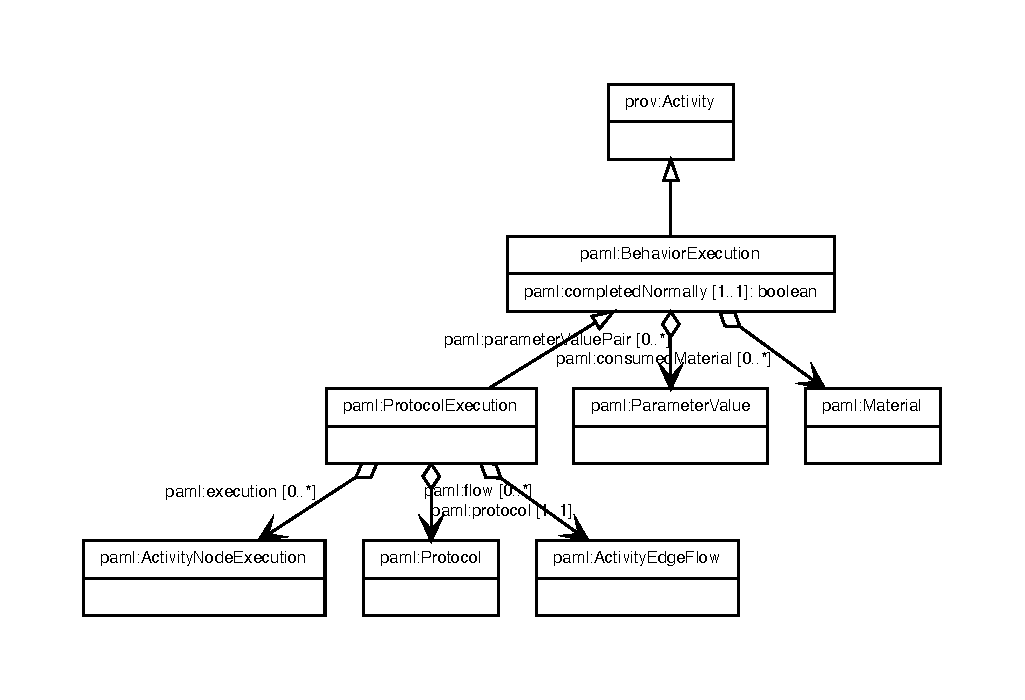
\includegraphics[width=0.7327659574468085\textwidth]{labop_classes/BehaviorExecution_abstraction_hierarchy.pdf}%
\caption{BehaviorExecution}%
\label{fig:BehaviorExecution}%
\end{figure}

%
The \labop{BehaviorExecution} class is shown in \ref{fig:BehaviorExecution}. It is derived from \prov{Activity} and includes the following specializations: \labop{ProtocolExecution}. %
This class includes the following properties: \labop{completedNormally}, \labop{parameterValuePair}, \labop{consumedMaterial}. %
\begin{itemize}%
\item%
The \labop{parameterValuePair} property is OPTIONAL and contains URI references to associated objects of type ParameterValueThe parameterValuePair property is used to record the value that was associated with each
        uml:Parameter for the uml:Behavior when it was executed, by means of a ParameterValue object.
        Any uml:Parameter that is not listed is assumed to have had no value assigned. Conversely, every non-optional
        uml:Parameter for the uml:Behavior MUST have an associated parameter value.
        Finally, note that this applies both to input uml:Parameter objects, whose value is set before execution begins,
        and to output uml:Parameter objects, whose value is set by the time execution ends.

        TODO: are multiple values allowed, or do those need to be passed as list/set types?
        %
\item%
The \labop{consumedMaterial} property is OPTIONAL and contains URI references to associated objects of type MaterialThis property is used to record the noteworthy consumables used during the execution of the
        Behavior. For example, a cell culture protocols will consume various reagents and samples of cells. Materials
        with the same specification SHOULD be consolidated, such that the list of materials SHOULD NOT contain two
        materials with the same specification.

        For example, consuming 5.0 mL of PBS and 2.0 mL of PBS should be recorded as consuming 7.0 mL of PBS.
        Complex materials, however, MAY contain the same material more than once in their substructure.
        For example, M9 media contains glucose, but it would not be necessary to consolidate the glucose in M9 media
        with additional glucose that was added as a supplement, since that would change the definition of the media.%
\item%
The \labop{completedNormally} property is REQUIRED and has a singleton value of type booleanThis boolean should be set to true if the Behavior completed normally and false if there
        was some exception condition. At present, no further information is being encoded about exceptions, but this
        is an extension that is anticipated for the future.%
\end{itemize}%
\subsubsection{ProtocolExecution}%
\label{sec:labop:ProtocolExecution}%
A \labop{ProtocolExecution} expands on the information in a \labop{BehaviorExecution} by including records for
        the nodes and edges defining the Protocol's behavior as a \uml{Activity}. Specifically, the execution property
        is used to record each firing of a \uml{ActivityNode} and the flow property is used to record each time a token
        moves along a \uml{ActivityEdge}.
        Otherwise, a \labop{ProtocolExecution} is used exactly the same way as its parent class \labop{BehaviorExecution}.

        TODO: consider dropping the protocol field as redundant with use prov:type field in its parent%
\newline%
\linebreak%
The \labop{ProtocolExecution} class is shown in \ref{fig:BehaviorExecution}. It is derived from \labop{BehaviorExecution}.%
This class includes the following properties: \labop{execution}, \labop{protocol}, \labop{flow}. %
\begin{itemize}%
\item%
The \labop{execution} property is OPTIONAL and contains URI references to associated objects of type ActivityNodeExecutionEach instance of this property links to an ActivityNodeExecution that records one
        firing of a uml:ActivityNode during the execution of its containing Protocol%
\item%
The \labop{protocol} property is REQUIRED and contains a URI reference to an associated object of type ProtocolThis property appears to be redundant with the use of prov:type specified by BehaviorExecution, and is likely to be deleted%
\item%
The \labop{flow} property is OPTIONAL and contains URI references to associated objects of type ActivityEdgeFlowEach instance of this property links to an ActivityEdgeFlow that records one movement of a UML
        token along a uml:ActivityEdge during the execution of its containing Protocol%
\end{itemize}%
\subsection{ParameterValue}%
\label{sec:labop:ParameterValue}%
This class is used to represent the assignment of a value to a parameter in a BehaviorExecution
        that records the execution of a \uml{Behavior}. This class is similar to \prov{Usage}, but instead of always
        pointing to an object it uses an arbitrary literal (which might or might not be an object). An example would
        be recording that a plate reader absorbance measurement was taken with its absorbance wavelength parameter set
        to 600 nm%
\newline%
\linebreak%


\begin{figure}[h!]%
\centering%
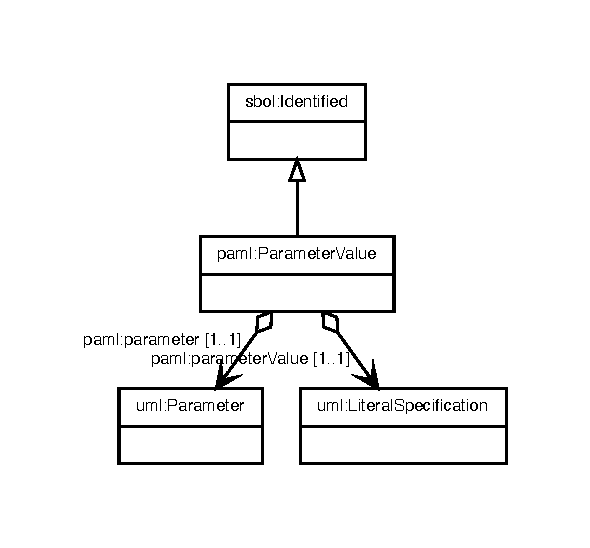
\includegraphics[width=0.42148936170212764\textwidth]{labop_classes/ParameterValue_abstraction_hierarchy.pdf}%
\caption{ParameterValue}%
\label{fig:ParameterValue}%
\end{figure}

%
The \labop{ParameterValue} class is shown in \ref{fig:ParameterValue}. It is derived from \sbol{Identified}.%
This class includes the following properties: \labop{parameter}, \labop{parameterValue}. %
\begin{itemize}%
\item%
The \labop{parameter} property is REQUIRED and contains a URI reference to an associated object of type ParameterThis property points to the uml:Parameter associated with the value (e.g., wavelength for a
        plate reader absorbance measurement behavior).%
\item%
The \labop{parameterValue} property is REQUIRED and contains a URI reference to an associated object of type LiteralSpecificationThis property points to the literal value used for the parameter during execution (e.g., a
        uml:LiteralIdentified for an om:Measure representing a 600 nm wavelength).%
\end{itemize}%
\subsection{Material}%
\label{sec:labop:Material}%
An amount of material allocated for use during the execution of a behavior.
        For example a \labop{Material} might be used to specify 1 96-well flat-bottom microplate or 2.5 mL of 10 millimolar glucose.

        TODO: consider changing type of specification to allow non-TopLevel descriptions, such as a \labop{ContainerSpec} or sbol:ExternallyDefined
        TODO: consider adding a field to distinguish between expended vs. reusable materials.%
\newline%
\linebreak%


\begin{figure}[h!]%
\centering%
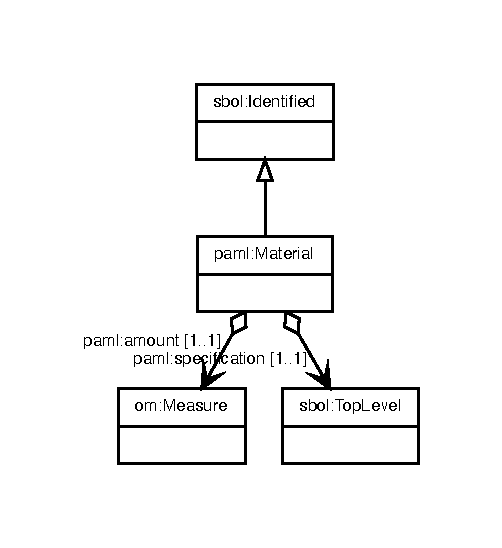
\includegraphics[width=0.35893617021276597\textwidth]{labop_classes/Material_abstraction_hierarchy.pdf}%
\caption{Material}%
\label{fig:Material}%
\end{figure}

%
The \labop{Material} class is shown in \ref{fig:Material}. It is derived from \sbol{Identified}.%
This class includes the following properties: \labop{amount}, \labop{specification}. %
\begin{itemize}%
\item%
The \labop{amount} property is REQUIRED and contains a URI reference to an associated object of type MeasureThe amount property of a Material is used to indicate the quantity of material used.
        For example, 2.5 mL (referring to a fluid) or 3 (with unit "number", referring to a group of microplates)%
\item%
The \labop{specification} property is REQUIRED and contains a URI reference to an associated object of type TopLevelThe specification property is used to indicate the type of material used.
        For example a DNA sample would be described by an sbol:Component.

        TODO: add example for glucose and for 96-well plate%
\end{itemize}%
\subsection{ActivityEdgeFlow}%
\label{sec:labop:ActivityEdgeFlow}%
An \labop{ActivityEdgeFlow} records \sbol{one} movement of a UML token along a \uml{ActivityEdge} during the
        execution of its containing \labop{Protocol}. If the edge is a \uml{ObjectFlow}, then the value MUST be set.
        If the edge is a \uml{ControlFlow}, then the value MUST NOT be set.

        For instance, the \labop{ActivityEdgeFlow} for a \uml{ObjectFlow} might record a measurement being sent to an output
        \uml{Parameter}, while the \labop{ActivityEdgeFlow} for a \uml{ControlFlow} might record a decision to proceed down a
        particular branch from a \uml{DecisionNode}.

        Note that a \uml{ActivityEdge} might appear in multiple \labop{ActivityEdgeFlow} records associated with a single
        \labop{ProtocolExecution}, e.g., due to a loop in the \labop{Protocol}.  It also might not appear in any, if the
        \uml{ActivityEdge} is on a path not taken due to branching control flow.

        TODO: correct the cardinality: edgeValue is supposed to be optional, not edge
        %
\newline%
\linebreak%


\begin{figure}[h!]%
\centering%
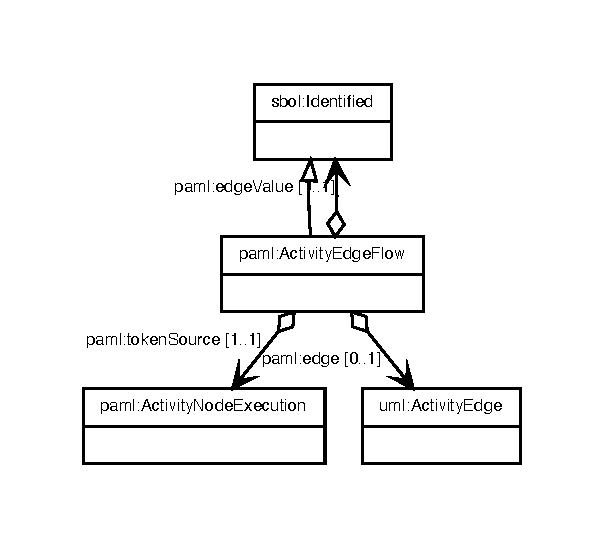
\includegraphics[width=0.4319148936170213\textwidth]{labop_classes/ActivityEdgeFlow_abstraction_hierarchy.pdf}%
\caption{ActivityEdgeFlow}%
\label{fig:ActivityEdgeFlow}%
\end{figure}

%
The \labop{ActivityEdgeFlow} class is shown in \ref{fig:ActivityEdgeFlow}. It is derived from \sbol{Identified}.%
This class includes the following properties: \labop{tokenSource}, \labop{edge}, \labop{edgeValue}. %
\begin{itemize}%
\item%
The \labop{tokenSource} property is REQUIRED and contains a URI reference to an associated object of type ActivityNodeExecutionThis property is used to indicate the ActivityNodeExecution that produced the token.%
\item%
The \labop{edge} property is OPTIONAL and contains a URI reference to an associated object of type ActivityEdgeThis property is used to indicate the uml:ActivityEdge down which the token moved.%
\item%
The \labop{edgeValue} property is REQUIRED and contains a URI reference to an associated object of type IdentifiedThis property is used to indicate the value of a token that moved on a uml:ObjectFlow edge.%
\end{itemize}%
\subsection{ActivityNodeExecution}%
\label{sec:labop:ActivityNodeExecution}%
An \labop{ActivityNodeExecution} records \sbol{one} instance in which a \uml{ActivityNode} is executed during the
        execution of its containing \labop{Protocol}.

        For instance, the \labop{ActivityNodeExecution} for a \uml{CallBehaviorAction} to measure absorbance on a plate reader
        would set its node property to point to the \uml{CallBehaviorAction} and might have incomingFlow properties
        indicating arrival of information about the samples to measure via a \uml{ObjectFlow} and the arrival a
        of permission to begin via a \uml{ControlFlow}.

        Note that a \uml{ActivityNode} might appear in multiple \labop{ActivityNodeExecution} records associated with a single
        \labop{ProtocolExecution}, e.g., due to a loop in the \labop{Protocol}.  It also might not appear in any, if the
        \uml{ActivityNode} is on a path not taken due to branching control flow.%
\newline%
\linebreak%


\begin{figure}[h!]%
\centering%
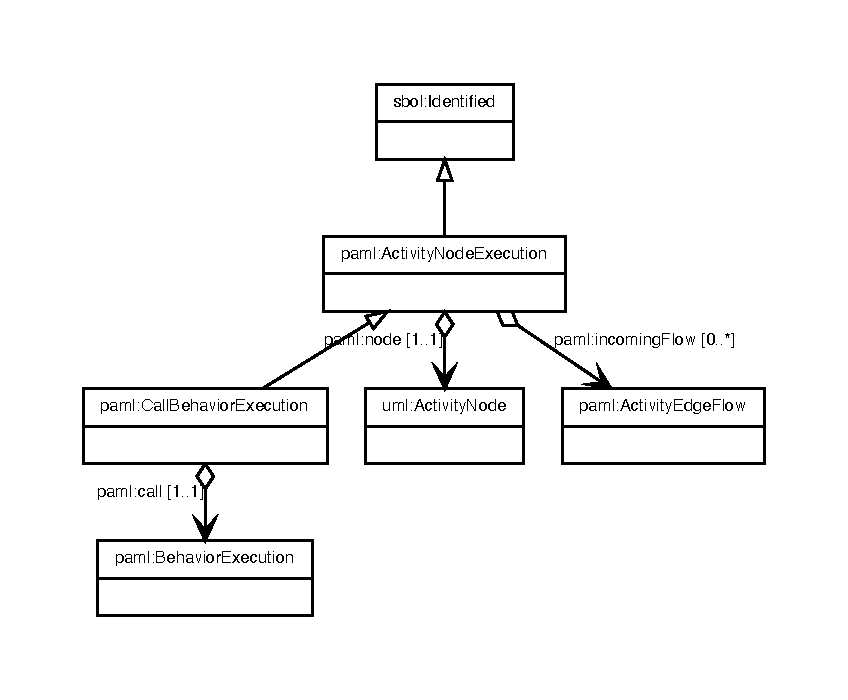
\includegraphics[width=0.6061702127659574\textwidth]{labop_classes/ActivityNodeExecution_abstraction_hierarchy.pdf}%
\caption{ActivityNodeExecution}%
\label{fig:ActivityNodeExecution}%
\end{figure}

%
The \labop{ActivityNodeExecution} class is shown in \ref{fig:ActivityNodeExecution}. It is derived from \sbol{Identified} and includes the following specializations: \labop{CallBehaviorExecution}. %
This class includes the following properties: \labop{node}, \labop{incomingFlow}. %
\begin{itemize}%
\item%
The \labop{node} property is REQUIRED and contains a URI reference to an associated object of type ActivityNodeThis property is used to indicate the uml:ActivityNode that has been execcuted.%
\item%
The \labop{incomingFlow} property is OPTIONAL and contains URI references to associated objects of type ActivityEdgeFlowThis property is used to indicate an ActivityEdgeFlow that delivered a token consumed during
        the execution of the uml:ActivityNode.%
\end{itemize}%
\subsubsection{CallBehaviorExecution}%
\label{sec:labop:CallBehaviorExecution}%
A \labop{CallBehaviorExecution} extends \labop{ActivityNodeExecution} by adding a pointer to a BehaviorExecution
        record for the \uml{Behavior} that is being executed.

        For a primitive action (e.g., measuring absorbance on a plate reader), this is a plain \labop{BehaviorExecution},
        while for calling a \labop{Protocol} as a sub-routine (e.g., to run a stage of an Type IIS assembly), this would be a
        \labop{ProtocolExecution}.%
\newline%
\linebreak%
The \labop{CallBehaviorExecution} class is shown in \ref{fig:ActivityNodeExecution}. It is derived from \labop{ActivityNodeExecution}.%
This class includes the following properties: \labop{call}. %
\begin{itemize}%
\item%
The \labop{call} property is REQUIRED and contains a URI reference to an associated object of type BehaviorExecutionThis property indicates the BehaviorExecution record for the uml:Behavior that was called.%
\end{itemize}%
\subsection{SampleCollection}%
\label{sec:labop:SampleCollection}%
SampleCollection is the base class for describing the collections of physical materials that are
         acted upon by a \labop{Protocol}. For example, a \labop{SampleCollection} might describe a set of 10 cell cultures growing in
         96-well plate cells, or a set of 6 streaked agar plates, or a single 500 mL flask filled with media.

         There are two types of \labop{SampleCollection}. A \labop{SampleArray} specifies an n-dimensional rectangular array of samples,
         all stored in the same type of container. A \labop{SampleMask} specifies a subset of a \labop{SampleCollection} by means of an
         array of Boolean values indicating whether each element is included or excluded from the subset.

         Note, however, that a \labop{SampleCollection} is a logical object and not a physical object. Thus, while a
         \labop{SampleCollection} might describe a set of samples in 96-well plate wells, it does not necessarily identify
         a particular 96-well plate or the location of those wells.  In practice, these will be determined as a
         result of the specific library calls made to generate \labop{SampleCollection} objects, and may not be determined
         until the protocol is actually run in a particular execution environment.

         This is important for increasing the flexibility with which a \labop{Protocol} can be specified and applied.
         Consider, for example, a cell culturing protocol that includes a step to measure \sbol{sample} absorbance on a plate
         reader. Describing this step does not require knowing how the samples are laid out on the plate, and in many
         cases is even acceptable to run on samples across multiple plates. This flexibility will allow the cell
         culturing protocol to be applied for experiments with different numbers and arrangements of samples.%
\newline%
\linebreak%


\begin{figure}[h!]%
\centering%
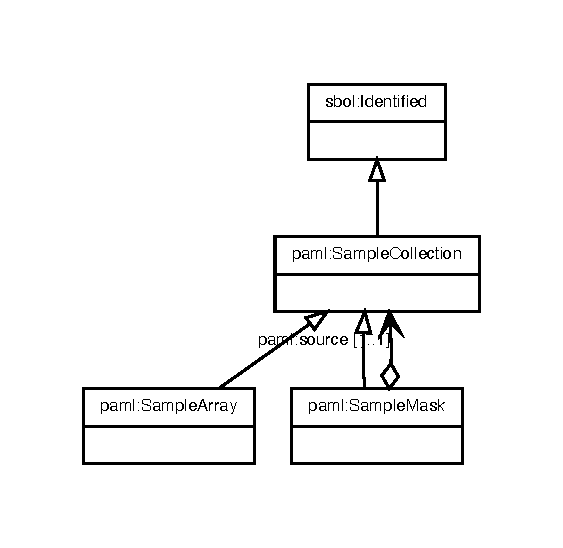
\includegraphics[width=0.40212765957446805\textwidth]{labop_classes/SampleCollection_abstraction_hierarchy.pdf}%
\caption{SampleCollection}%
\label{fig:SampleCollection}%
\end{figure}

%
The \labop{SampleCollection} class is shown in \ref{fig:SampleCollection}. It is derived from \sbol{Identified} and includes the following specializations: \labop{SampleArray}, \labop{SampleMask}. %
%
\subsubsection{SampleArray}%
\label{sec:labop:SampleArray}%
A \labop{SampleArray} specifies an n-dimensional rectangular array of samples, all stored in the same
        type of container. For example, a \labop{SampleCollection} might describe a set of 10 cell cultures growing in
        96-well plate cells, or a set of 6 streaked agar plates, or a single 500 mL flask filled with media.

        Wells may be full, in which case the contents property should contain a URI to a description of the \sbol{sample},
        or empty, in which case the contents should be null.

        Note that this is a logical array, and does not necessarily indicate the actual layout of the samples in space.
        For example, a 2x4 array of samples in 96-well plate wells might end up being laid out as a 2x4 array in wells
        A1 to B4 or as a 2x4 array in wells G5 to H8 or as an 8x1 column in wells A1 to H1, or even as eight wells
        scattered arbitrarily around the plate according to an anti-bias quality control schema.

        This also allows for higher-dimensional arrays where each dimension represents an experimental factor.
        For example, an experiment testing four factors with 3, 3, 4, and 5 values per factor, for a total of 180
        combinations, could be represented as a 4-dimensional \sbol{sample} array of 96-well plate wells, and then end up
        laid out over two plates.

        TODO: need to decide on the format of the contents description.%
\newline%
\linebreak%
The \labop{SampleArray} class is shown in \ref{fig:SampleCollection}. It is derived from \labop{SampleCollection}.%
This class includes the following properties: \labop{contents}, \labop{containerType}. %
\begin{itemize}%
\item%
The \labop{contents} property is REQUIRED and has a singleton value of type stringDescription of the contents.
        TODO: need to decide whether this is a multi-valued property with associated array coordinates or a
        single-valued property with an array value.
        Currently set to string as a "dummy" value that can serialize anything.%
\item%
The \labop{containerType} property is REQUIRED and has a singleton value of type URI%
\end{itemize}%
\subsubsection{SampleMask}%
\label{sec:labop:SampleMask}%
A \labop{SampleMask} is a subset of a \labop{SampleCollection}. The subset of samples to be included is defined
        by an array of Boolean values, where true values indicate that a \sbol{sample} is included and false values indicate
        that it is excluded.

        The dimensions of the mask MUST be identical to the dimensions of the source \labop{SampleCollection}. For this purpose,
        the dimensions of a masked subset are not reduced, but remain the same as the original \labop{SampleArray}. This allows
        masks to be composed, such that SampleMask(source=SampleMask(source=X,mask=mask1),mask=mask2) is equivalent to
        SampleMask(source=X,mask=mask1 AND mask2). Note that this implies masks are commutative and idempotent.%
\newline%
\linebreak%
The \labop{SampleMask} class is shown in \ref{fig:SampleCollection}. It is derived from \labop{SampleCollection}.%
This class includes the following properties: \labop{mask}, \labop{source}. %
\begin{itemize}%
\item%
The \labop{source} property is REQUIRED and contains a URI reference to an associated object of type SampleCollectionThe source indicates the SampleCollection that is being subsetted via the mask%
\item%
The \labop{mask} property is REQUIRED and has a singleton value of type stringThe mask is an N-dimensional array of Booleans values, where each Boolean indicates whether the
        sample at the corresponding location in the source is included in the subset.

        TODO: format of mask array needs to match the array format chosen for the SampleArray contents property%
\end{itemize}%
\subsection{SampleData}%
\label{sec:labop:SampleData}%
The \labop{SampleData} class is used to associate a set of data with a collection of samples.
        This is typically used to capture measurements, e.g., an array of absorbance measurements collected by
        a plate reader. Using this data structure allows the values in a dataframe to be automatically linked to
        the descriptions of the samples that the data describes, which is critical for data analysis.

        The dimensions of the sampleDataValues MUST equal the dimensions of the \labop{SampleCollection} linked with fromSamples.

        TODO: the format of the data values needs to be compatible with the array format chosen for the
        \labop{SampleArray} contents property. In this case, however, we also need to consider how we want to support
        multiple values for each \sbol{sample} (e.g., measurement of both fluorescence and absorbance in a plate reader),
        as well as links to more complex data (e.g., results of flow cytometry or omics for each sample)%
\newline%
\linebreak%


\begin{figure}[h!]%
\centering%
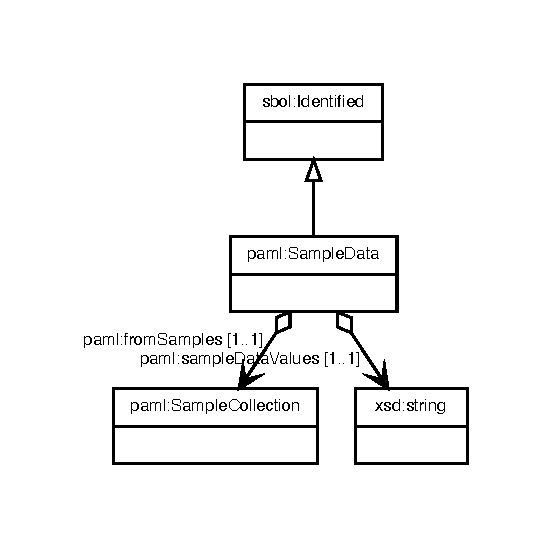
\includegraphics[width=0.3946808510638298\textwidth]{labop_classes/SampleData_abstraction_hierarchy.pdf}%
\caption{SampleData}%
\label{fig:SampleData}%
\end{figure}

%
The \labop{SampleData} class is shown in \ref{fig:SampleData}. It is derived from \sbol{Identified}.%
This class includes the following properties: \labop{fromSamples}, \labop{sampleDataValues}. %
\begin{itemize}%
\item%
The \labop{fromSamples} property is REQUIRED and contains a URI reference to an associated object of type SampleCollectionThe fromSamples property indicates the SampleCollection from which the data were collected.%
\item%
The \labop{sampleDataValues} property is REQUIRED and contains a URI reference to an associated object of type stringThe sampleDataValues are an array of data values, one for each sample, format to be determined.%
\end{itemize}%
\subsection{ContainerSpec}%
\label{sec:labop:ContainerSpec}%
A \labop{ContainerSpec} is used to indicate the type of container to be used for a \labop{SampleArray}, e.g.,
        a standard 96-well flat-bottom transparent plate.

        TODO: determine if we want to use this format or modify it in some way.%
\newline%
\linebreak%


\begin{figure}[h!]%
\centering%
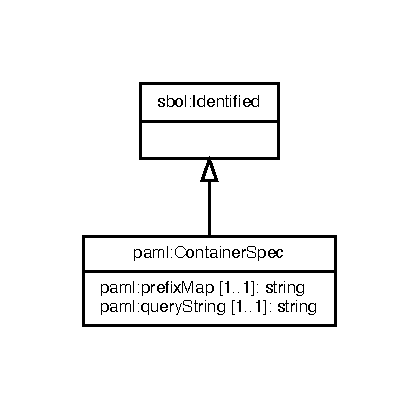
\includegraphics[width=0.29936170212765956\textwidth]{labop_classes/ContainerSpec_abstraction_hierarchy.pdf}%
\caption{ContainerSpec}%
\label{fig:ContainerSpec}%
\end{figure}

%
The \labop{ContainerSpec} class is shown in \ref{fig:ContainerSpec}. It is derived from \sbol{Identified}.%
This class includes the following properties: \labop{prefixMap}, \labop{queryString}. %
\begin{itemize}%
\item%
The \labop{prefixMap} property is REQUIRED and has a singleton value of type stringA prefix map in JSON-LD format, to be applied to a queryString.%
\item%
The \labop{queryString} property is REQUIRED and has a singleton value of type stringA query string, in OWL Manchester syntax, to be used to find matching containers in the ContainerSpec.%
\end{itemize}%


\section{Serialization}
\label{sec:serialization}

In order for PAML objects to be readily stored and exchanged, it is important that they are able to be {\em serialized}, i.e., converted to a sequence of bytes that can be stored in a file or exchanged over a network.  
%
To this end, PAML builds upon the Resource Description Framework (RDF).  RDF is an abstract language for describing conceptual graph-oriented data models, and therefore does not mandate any specific serialization format.  Instead, a number of different serialization formats are provided as separate specifications, such as RDF/XML, N-Triples, JSON-LD, and Turtle.  These serialization formats are widely supported by RDF libraries such as rdflib for Python and Apache Jena for Java.

All PAML libraries SHOULD support at least RDF/XML, N-Triples, JSON-LD, and Turtle.
Other PAML tools SHOULD support at least one of these four formats.


\newpage
\bibliography{labop}

\appendix

%\input{examples}

\end{document}
